\chapter[$\mathcal{H}_2$ Performance of Cyclic Networks]{$\mathcal{H}_2$ Performance of a Network of Double-Integrators in Presence of Cycles}\label{ch:Robustness_Analysis}
\section{Introduction}\label{sec:ch_RA_intro}
While Chapter \ref{ch:Guaranteed_Consensus} formulated deterministic local remedies to prevent dynamic divergence and guarantee consensus over a directed network of double-integrators, guaranteeing bounded state agreement is only a baseline requirement. In real-world physical deployments, such as autonomous vehicular platoons and airborne formations subject to wind gusts or sensor noise, multi-agent systems operate under disturbances and noises. Consequently, evaluating how measurement noise and process perturbations propagate across cyclic graphs, using input-output performance metrics such as the $\mathcal{H}_2$ norm, becomes an essential design objective.

Up to this point, our investigations in Chapters \ref{ch:TwoReverseEdges} and \ref{ch:Guaranteed_Consensus} focused exclusively on \emph{directed} communication topologies. In this chapter, we resort to analyzing performance over \emph{undirected} graphs. While undirected networks feature symmetric Laplacian matrices with real spectra, extending $\mathcal{H}_2$ norm performance analysis to second-order agents over undirected cyclic graphs exposes deep, non-trivial combinatorial challenges that do not reveal themselves when agents are modeled as single integrators. Given the rich structural interactions between second-order momentum terms, graph combinatorial properties, and noise propagation, establishing a thorough analytical foundation for undirected double-integrator systems is a necessary and significant prerequisite towards tackling the broader complexity of directed $\mathcal{H}_2$ performance metrics.

A fundamental challenge in evaluating the $\mathcal{H}_2$ performance of consensus protocols is the presence of the zero Laplacian eigenvalue ($\lambda_1 = 0$), which causes the standard controllability Gramian to be unbounded. For single-integrator networks, Zelazo et al. \cite{zelazo2010edge, zelazo2013performance} resolved this singularity using an edge-space projection over reduced-order trees, establishing that adding cycles strictly improves the $\mathcal{H}_2$ norm, quite agnostic to the choice of spanning tree or the spatial location of the cycle. 

However, physical mechanical platforms are governed by Newton's second law of motion, where physical force or acceleration serves as the control input. Extending $\mathcal{H}_2$ performance analysis to double-integrator networks introduces complex cross-coupling between relative position alignment and physical velocity damping. Because double integrators store energy in velocity states, their performance sensitivity to combinatorial graph properties— such as spatial cycle placement and edge overlap— diverges fundamentally from first-order kinematic models. Even under symmetric undirected topologies, double-integrator networks exhibit a strong sensitivity to \emph{where} a cycle is placed and \emph{how much} two cycles overlap— spatial dependencies that are absent in single-integrator consensus.

%While Chapter \ref{ch:Guaranteed_Consensus} formulated deterministic local remedies to prevent dynamic divergence and guarantee consensus stability in double-integrator networks, guaranteeing bounded state agreement is only a baseline requirement. In real-world physical deployments— such as autonomous vehicular platoons and airborne formations subject to wind gusts or sensor drift, multi-agent systems operate under disturbances. Consequently, evaluating how measurement noise and process perturbations propagate across cyclic communication graphs using input-output performance metrics, such as the $\mathcal{H}_2$ norm, becomes an essential design objective.

\subsection*{Summary of Chapter Contributions}
This chapter addresses the aforesaid gap by establishing an exact analytical $\mathcal{H}_2$ performance framework for double-integrators over an undirected network containing cycle(s). The main contributions of this chapter are:
\begin{enumerate}
    \item \textbf{Exact Closed-Form $\mathcal{H}_2$ Norm Expression:} By constructing an edge-space projection $\Sigma_e$ that decouples the unobservable rigid-body drift modes, we derive the exact, closed-form solution to the 2x2 block Lyapunov equation, proving that a double-integrator network always exhibits a larger $\mathcal{H}_2$ norm (poorer noise attenuation) than a single-integrator network.
    \item \textbf{Spanning Tree and Sensitivity to Placement in Network:} Unlike single-integrator systems (where all spanning trees and cycle locations yield identical $\mathcal{H}_2$ performance), we prove that for double integrators, the $\mathcal{H}_2$ norm does depend on the choice of spanning tree and the spatial location of the cycle within the graph. Specifically, placing a cycle near the spatial center of a path graph reduces the system's $\mathcal{H}_2$ norm.
    \item \textbf{Optimal Two-Cycle Overlap Bound:} For networks containing two interacting cycles, we utilize Jensen's Inequality to prove that completely non-overlapping cycles are suboptimal. We derive exact analytical upper bounds on the extent of edge overlap $s \coloneqq  k_1 + k_2$ that guarantees optimal noise suppression.
\end{enumerate}
\section{Graph-Theoretic Preliminaries and Edge Factorizations}\label{sec:ch4_preliminaries}
Let $\mathcal{G} = (\mathcal{V}, \mathcal{E})$ denote a connected, undirected graph with vertex set $\mathcal{V}$ ($|\mathcal{V}| = n$) and edge set $\mathcal{E}$ ($|\mathcal{E}| = e$). Assigning an arbitrary orientation to each edge $k = (i,j) \in \mathcal{E}$, the incidence matrix $E(\mathcal{G}) \in \mathbb{R}^{n \times e}$ is defined component-wise as:
\begin{equation}\label{eq:ch_RA_incidence_def}
	[E(\mathcal{G})]_{ik} = \begin{cases}
		+1, & \text{if vertex } i \text{ is the head of edge } k \\
		-1, & \text{if vertex } i \text{ is the tail of edge } k \\
		0, & \text{otherwise}
	\end{cases}
\end{equation}
The graph Laplacian matrix $\mathcal{L} \in \mathbb{R}^{n \times n}$ is factored as $\mathcal{L} = E(\mathcal{G}) E(\mathcal{G})^T$. 

Select a spanning tree $\mathcal{T} \subset \mathcal{G}$ consisting of $n-1$ tree edges. Partition the incidence matrix as $E(\mathcal{G}) = \begin{bmatrix} E_\tau & E_c \end{bmatrix}$, where $E_\tau \in \mathbb{R}^{n \times (n-1)}$ contains the columns corresponding to spanning tree edges, and $E_c \in \mathbb{R}^{n \times (e-n+1)}$ contains the remaining $e-n+1$ cycle-closing edges. Since the columns of $E_c$ lie in the column space of $E_\tau$, we express $E_c = E_\tau T$, where $T \in \mathbb{R}^{(n-1) \times (e-n+1)}$ is the cycle-basis matrix given by:
\begin{equation}\label{eq:ch_RA_T_matrix}
	T \coloneqq (E_\tau^T E_\tau)^{-1} E_\tau^T E_c
\end{equation}
This yields the fundamental incidence matrix factorization \cite{godsil2001algebraic, zelazo2013performance}:
\begin{equation}\label{eq:ch_RA_incidence_factorization}
	E(\mathcal{G}) = E_\tau \begin{bmatrix} I_{n-1} & T \end{bmatrix} \eqcolon E_\tau R, \quad \text{where } R \coloneqq \begin{bmatrix} I_{n-1} & T \end{bmatrix} \in \mathbb{R}^{(n-1) \times e}
\end{equation}

The tree edge Laplacian $\letree \in \mathbb{R}^{(n-1) \times (n-1)}$ is defined as $\letree \coloneqq E_\tau^T E_\tau$. The essential edge Laplacian $A_3 \in \mathbb{R}^{(n-1) \times (n-1)}$ is defined as:
\begin{equation}\label{eq:ch_RA_A3_def}
	A_3 \coloneqq \letree R R^T = E_\tau^T E(\mathcal{G}) E(\mathcal{G})^T E_\tau (E_\tau^T E_\tau)^{-1}
\end{equation}
Observe that matrix $A_3$ is symmetric, positive definite, and contains all the $(n-1)$ non-zero eigenvalues of the graph Laplacian $\mathcal{L}$.



\section{System Dynamics and Edge-Space Realization}\label{sec:ch_RA_problem_formulation}
In this section, we formulate the noisy state-space model for a networked multi-agent system of double integrators subject to exogenous process disturbances and relative measurement noise. We then construct an explicit coordinate transformation onto an edge-based subspace, eliminating the unobservable rigid-body consensus modes and yielding a minimal, reduced-order realization suitable for $\mathcal{H}_2$ norm computation.

\subsection{Double-Integrator Consensus Model under Noise}

Consider an undirected graph $\mathcal{G} = (\mathcal{V}, \mathcal{E})$ consisting of $n = |\mathcal{V}|$ identical double-integrator agents connected by $e = |\mathcal{E}|$ communication links. The physical translational motion of agent $i \in \{1, 2, \dots, n\}$ is subject to zero-mean, uncorrelated Gaussian process noise $q_i(t) \in \mathbb{R}$ with variance $\mathbb{E}[q_i(t) q_i^T(\tau)] = \sigma_q^2 \delta(t - \tau)$:
\begin{equation}\label{eq:ch_RA_agent_dynamics}
	\dot{x}_i(t) = v_i(t), \quad \dot{v}_i(t) = u_i(t) + q_i(t), \quad i \in \{1, 2, \dots, n\}
\end{equation}
where $x_i(t), v_i(t) \in \mathbb{R}$ denote the scalar position and velocity states of agent $i$, and $u_i(t) \in \mathbb{R}$ represents the control input.

To achieve state agreement over $\mathcal{G}$, agents exchange relative position and relative velocity states with their immediate spatial neighbors. In practical deployments, edge communication channels are corrupted by zero-mean Gaussian measurement noise $r_{ij}(t) \in \mathbb{R}$ with variance $\mathbb{E}[r_{ij}(t) r_{ij}^T(\tau)] = \sigma_r^2 \delta(t - \tau)$. The localized control law $u_i(t)$ incorporating relative measurement noise is defined as:
\begin{equation}\label{eq:ch_RA_control_law}
	u_i(t) = \sum_{j=1}^{n} a_{ij} \left[ (x_j(t) - x_i(t)) + \gamma (v_j(t) - v_i(t)) + r_{ij}(t) \right]
\end{equation}
where $a_{ij} \in \{0, 1\}$ represents the $(i,j)$-th entry of the unweighted adjacency matrix $\mathcal{W}$, and $\gamma > 0$ denotes the global velocity coupling parameter.

To express protocol \eqref{eq:ch_RA_control_law} in compact network coordinates, stack the individual node states, process disturbances, and edge measurement noise into global vectors:
\begin{equation}\label{eq:ch_RA_stackedstates}
	x(t) \coloneqq \begin{bmatrix} x_1(t) \\ \vdots \\ x_n(t) \end{bmatrix} \in \mathbb{R}^n, \quad 
	v(t) \coloneqq \begin{bmatrix} v_1(t) \\ \vdots \\ v_n(t) \end{bmatrix} \in \mathbb{R}^n, \quad 
\end{equation}
\begin{equation}\label{eq:ch_RA_stackednoises}
	q(t) \coloneqq \begin{bmatrix} q_1(t) \\ \vdots \\ q_n(t) \end{bmatrix} \in \mathbb{R}^n, \quad 
	r(t) \coloneqq \begin{bmatrix} r_1(t) \\ \vdots \\ r_e(t) \end{bmatrix} \in \mathbb{R}^e
\end{equation}

Recalling the incidence matrix $E(\mathcal{G}) \in \mathbb{R}^{n \times e}$ from Definition \ref{def:incidence_matrix}, the relative state vector across all $e$ edges can be written as $E^T x(t) \in \mathbb{R}^e$ and $E^T v(t) \in \mathbb{R}^e$. Consequently, the aggregated control vector $u(t) = [u_1(t), \dots, u_n(t)]^T \in \mathbb{R}^n$ expands as:
\begin{align}\label{eq:ch_RA_control_vector}
	u(t) &= -E E^T x(t) - \gamma E E^T v(t) - E r(t) \nonumber \\
	&= -\mathcal{L} x(t) - \gamma \mathcal{L} v(t) - E r(t)
\end{align}
where $\mathcal{L} = E E^T \in \mathbb{R}^{n \times n}$ is the standard graph Laplacian matrix.

Substituting \eqref{eq:ch_RA_control_vector} into the state dynamics \eqref{eq:ch_RA_agent_dynamics} yields the global state equations:
\begin{equation}\label{eq:ch_RA_global_state_eq}
	\begin{aligned}
		\dot{x}(t) &= v(t) \\
		\dot{v}(t) &= -\mathcal{L} x(t) - \gamma \mathcal{L} v(t) + q(t) - E r(t)
	\end{aligned}
\end{equation}

Defining the performance measurement signal $z(t) \in \mathbb{R}^{2e}$ as the vector of relative spatial and velocity displacements across all network edges ($z(t) \coloneqq [(E^T x(t))^T, (E^T v(t))^T]^T$), the full state-space system $\Sigma_n$ with composite state $X(t) \coloneqq [x^T(t), v^T(t)]^T \in \mathbb{R}^{2n}$ is given by:
\begin{equation}\label{eq:ch_RA_system_Sigman}
	\Sigma_n: \begin{cases}
		\dot{X}(t) = \begin{bmatrix} \mathbf{0}_{n \times n} & I_n \\ -\mathcal{L} & -\gamma \mathcal{L} \end{bmatrix} X(t) + \begin{bmatrix} \mathbf{0}_{n \times n} & \mathbf{0}_{n \times e} \\ I_n & -E \end{bmatrix} \begin{bmatrix} q(t) \\ r(t) \end{bmatrix} \\
		z(t) = \begin{bmatrix} E^T & \mathbf{0}_{e \times n} \\ \mathbf{0}_{e \times n} & E^T \end{bmatrix} X(t)
	\end{cases}
\end{equation}

\begin{figure}[ht!]
	\centering
	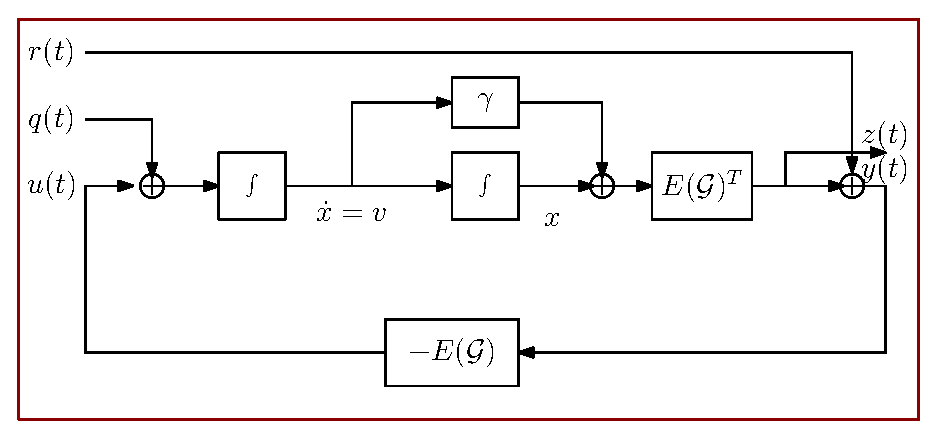
\includegraphics[scale=0.7]{4_Images/double_int_block_undirected.eps}
	\caption{Block diagram representation of the double-integrator network system $\Sigma_n$, depicting feedback loops, process noise $q(t)$, and edge measurement noise $r(t)$.}
	\label{fig:block_double}
\end{figure}
\subsection{Reduced-Order Edge-Space Realization}

System $\Sigma_n$ in \eqref{eq:ch_RA_system_Sigman} cannot be directly evaluated using standard $\mathcal{H}_2$ norm computation methods. Because the connected graph Laplacian $\mathcal{L}$ possesses a simple zero eigenvalue ($\lambda_1 = 0$) with right eigenvector $\mathbf{1}_n = [1, 1, \dots, 1]^T \in \mathbb{R}^n$, system $\Sigma_n$ contains two unobservable, non-stationary rigid-body modes corresponding to the average network position $\frac{1}{n} \mathbf{1}_n^T x(t)$ and average network velocity $\frac{1}{n} \mathbf{1}_n^T v(t)$. These drift modes cause the controllability Gramian of $\Sigma_n$ to be undefined ($X^* \to \infty$).

To project the network dynamics onto a stable subspace and eliminate these unobservable modes, we select a spanning tree $\mathcal{T} \subset \mathcal{G}$ consisting of $(n-1)$ tree edges. Using the incidence matrix factorization \eqref{eq:ch_RA_incidence_factorization} $E(\mathcal{G}) = E_\tau R = E_\tau \begin{bmatrix} I_{n-1} & T \end{bmatrix}$ from \eqref{eq:incidence_factored}, we introduce the linear spatial coordinate transformation matrix $S_v \in \mathbb{R}^{n \times n}$:
\begin{equation}\label{eq:ch_RA_transformation_Sv}
	S_v \coloneqq \begin{bmatrix} E_\tau (E_\tau^T E_\tau)^{-1} & \frac{1}{n} \mathbf{1}_n \end{bmatrix} = \begin{bmatrix} E_\tau \letree^{-1} & \frac{1}{n} \mathbf{1}_n \end{bmatrix}
\end{equation}
where $\letree = E_\tau^T E_\tau \in \mathbb{R}^{(n-1) \times (n-1)}$ is the positive-definite tree edge Laplacian matrix.

Applying $S_v$ to transform the nodal position and velocity vectors we have the following relationship:
\begin{equation}\label{eq:ch_RA_coordinate_change}
	x(t) = S_v x_e(t) = \begin{bmatrix} E_\tau \letree^{-1} & \frac{1}{n} \mathbf{1}_n \end{bmatrix} \begin{bmatrix} x_\tau(t) \\ x_\mathbf{1}(t) \end{bmatrix}, \quad 
	v(t) = S_v v_e(t) = \begin{bmatrix} E_\tau \letree^{-1} & \frac{1}{n} \mathbf{1}_n \end{bmatrix} \begin{bmatrix} v_\tau(t) \\ v_\mathbf{1}(t) \end{bmatrix}
\end{equation}
where $x_\tau(t) \coloneqq E_\tau^T x(t) \in \mathbb{R}^{n-1}$ and $v_\tau(t) \coloneqq E_\tau^T v(t) \in \mathbb{R}^{n-1}$ represent the relative position and velocity state vectors along the $n-1$ chosen spanning tree edges, while $x_\mathbf{1}(t) \coloneqq \mathbf{1}_n^T x(t) \in \mathbb{R}$ and $v_\mathbf{1}(t) \coloneqq \mathbf{1}_n^T v(t) \in \mathbb{R}$ denote the scalar centroid (average) modes.

Taking the inverse of transformation matrix $S_v$:
\begin{equation}\label{eq:ch_RA_Sv_inverse}
	S_v^{-1} = \begin{bmatrix} E_\tau^T \\ \mathbf{1}_n^T \end{bmatrix} \in \mathbb{R}^{n \times n},
\end{equation}
and pre-multiplying global state equations \eqref{eq:ch_RA_global_state_eq} by $S_v^{-1}$ separates out the relative edge coordinates as follows:.

\begin{enumerate}
	\item \textbf{Relative Tree Edge Dynamics ($x_\tau, v_\tau$):}
	\begin{align}\label{eq:ch_RA_edge_dynamics_raw}
		\dot{x}_\tau(t) &= E_\tau^T v(t) = v_\tau(t) \nonumber \\
		\dot{v}_\tau(t) &= E_\tau^T \dot{v}(t) = -E_\tau^T \mathcal{L} x(t) - \gamma E_\tau^T \mathcal{L} v(t) + E_\tau^T q(t) - E_\tau^T E r(t)
	\end{align}
	Substituting $\mathcal{L} = E E^T = E_\tau R R^T E_\tau^T$ into $E_\tau^T \mathcal{L} x(t)$:
	\begin{equation}
		E_\tau^T \mathcal{L} x(t) = (E_\tau^T E_\tau) R R^T (E_\tau^T x(t)) = \letree R R^T x_\tau(t) = A_3 x_\tau(t)
	\end{equation}
	where $A_3 \coloneqq \letree R R^T \in \mathbb{R}^{(n-1) \times (n-1)}$ is the essential edge Laplacian matrix introduced in \eqref{eq:ch_RA_A3_def}. Similarly, $E_\tau^T \mathcal{L} v(t) = A_3 v_\tau(t)$, and $E_\tau^T E r(t) = E_\tau^T E_\tau R r(t) = \letree R r(t)$. Thus:
	\begin{equation}\label{eq:ch_RA_v_tau_dot}
		\dot{v}_\tau(t) = -A_3 x_\tau(t) - \gamma A_3 v_\tau(t) + E_\tau^T q(t) - \letree R r(t)
	\end{equation}

	\item \textbf{Centroid Drift Dynamics ($x_\mathbf{1}, v_\mathbf{1}$):}
	\begin{align}\label{eq:ch_RA_centroid_dynamics}
		\dot{x}_\mathbf{1}(t) &= \mathbf{1}_n^T v(t) = v_\mathbf{1}(t) \nonumber \\
		\dot{v}_\mathbf{1}(t) &= \mathbf{1}_n^T \dot{v}(t) = -\mathbf{1}_n^T \mathcal{L} x(t) - \gamma \mathbf{1}_n^T \mathcal{L} v(t) + \mathbf{1}_n^T q(t) - \mathbf{1}_n^T E r(t)
	\end{align}
	Since $\mathbf{1}_n^T \mathcal{L} = \mathbf{0}^T$ and $\mathbf{1}_n^T E = \mathbf{0}^T$ for undirected graphs:
	\begin{equation}\label{centroid}
		\dot{x}_\mathbf{1}(t) = v_\mathbf{1}(t), \quad \dot{v}_\mathbf{1}(t) = \mathbf{1}_n^T q(t)
	\end{equation}
\end{enumerate}

Equations \eqref{eq:ch_RA_centroid_dynamics} and \eqref{centroid} confirm that the centroid state $x_\mathbf{1}(t)$ represents an unobservable mode driven purely by process noise $q(t)$, completely decoupled from the control law $u(t)$ and measurement noise $r(t)$.

Furthermore, transforming the output vector $z(t) = [(E^T x(t))^T~~ (E^T v(t))^T]^T$, we have:
\begin{equation}
	E^T x(t) = R^T E_\tau^T x(t) = R^T x_\tau(t), \quad E^T v(t) = R^T v_\tau(t).
\end{equation}
Since matrix $R^T \in \mathbb{R}^{e \times (n-1)}$ merely projects tree edge states onto all $e$ network edges, $z(t)$ contains redundant linearly dependent terms. Eliminating this output redundancy allows us to project output measurement $z(t)$ directly onto tree states $x_\tau(t)$ and $v_\tau(t)$.

Defining normalized white noise inputs $\hat{q}(t) \coloneqq q(t)/\sigma_q$ and $\hat{r}(t) \coloneqq r(t)/\sigma_r$, we isolate the minimal, asymptotically stable, reduced-order edge-space state vector $X_{e\tau}(t) \coloneqq [x_\tau^T(t), v_\tau^T(t)]^T \in \mathbb{R}^{2(n-1)}$:
\begin{equation}\label{eq:ch_RA_minimal_system_explicit}
	\Sigma: \begin{cases}
		\dot{X}_{e\tau}(t) = \begin{bmatrix} \mathbf{0}_{(n-1) \times (n-1)} & I_{n-1} \\ -A_3 & -\gamma A_3 \end{bmatrix} X_{e\tau}(t) + \begin{bmatrix} \mathbf{0}_{(n-1) \times n} & \mathbf{0}_{(n-1) \times e} \\ \sigma_q E_\tau^T & -\sigma_r \letree R \end{bmatrix} \begin{bmatrix} \hat{q}(t) \\ \hat{r}(t) \end{bmatrix} \\
		z(t) = X_{e\tau}(t)
	\end{cases}
\end{equation}

The minimal system $\Sigma$ in \eqref{eq:ch_RA_minimal_system_explicit} can be compactly represented by the transfer function matrix $G(s) = C (sI - A)^{-1} B$:
\begin{equation}\label{sigma_system}
	G(s) \coloneqq \left[ \begin{array}{c|c} A & B \\ \hline C & \mathbf{0} \end{array} \right]
\end{equation}
where the block state-space matrices are defined as:
\begin{equation}\label{eq:ch_RA_system_matrices_A}
	A \coloneqq \begin{bmatrix} \mathbf{0}_{(n-1) \times (n-1)} & I_{n-1} \\ 
    -A_3 & -\gamma A_3 \end{bmatrix} \in \mathbb{R}^{2(n-1) \times 2(n-1)},
\end{equation}
\begin{equation}\label{eq:ch_RA_system_matrices_B}
	B \coloneqq \begin{bmatrix} \mathbf{0}_{(n-1) \times n} & \mathbf{0}_{(n-1) \times e} \\ \sigma_q E_\tau^T & -\sigma_r \letree R \end{bmatrix} \in \mathbb{R}^{2(n-1) \times (n+e)}
\end{equation}
and $C \coloneqq I_{2(n-1)}$. Because $A_3 = \letree R R^T$ contains $(n-1)$ eigenvalues of the Laplacian, while leaving out the one eigenvalue at zero, for any connected graph $\mathcal{G}$, every eigenvalue of matrix $A$ possesses a strictly negative real part for all $\gamma > 0$. Thus, matrix $A$ is strictly Hurwitz, guaranteeing that minimal realization $\Sigma$ is asymptotically stable and that its $\mathcal{H}_2$ norm $\|\Sigma\|_2^2$ is bounded and well-defined.

\section{Analytical $\mathcal{H}_2$ Performance Characterization}\label{sec:ch_RA_MainResults}

The $\mathcal{H}_2$ norm of the reduced system $\Sigma$ measures the total output energy under unit-variance Gaussian noise inputs:
\begin{equation}\label{eq:ch_RA_H2_def}
	\|\Sigma\|_2^2 \coloneqq \text{trace}(X^*)
\end{equation}
where $X^* \in \mathbb{R}^{2(n-1) \times 2(n-1)}$ is the unique positive-definite solution to the state-space Lyapunov equation:
\begin{equation}\label{eq:ch_RA_lyapunov_eq}
	A X^* + X^* A^T + B B^T = 0
\end{equation}
with input matrix $B = \begin{bmatrix} \mathbf{0} & \mathbf{0} \\ \sigma_q E_\tau^T & -\sigma_r \letree R \end{bmatrix}$.

\begin{theo}[ $\mathcal{H}_2$ Norm for Network of Double-Integrators]\label{theoH2}
\leavevmode\par\noindent
Consider an undirected multi-agent network of double integrators governed by minimal edge system $\Sigma$ in \eqref{eq:ch_RA_minimal_system_explicit}. The $\mathcal{H}_2$ norm is given by the following expression:
\begin{equation}\label{total_norm}
	\|\Sigma\|_2^2 = \frac{1}{2\gamma} \text{trace}\left[ (I_{n-1} - A_3^{-1}) (\sigma_r^2 I_{n-1} - \sigma_q^2 A_3^{-1}) \letree \right].
\end{equation}
Expanding \eqref{total_norm} yields the explicit structural representation:
\begin{equation}\label{total_norm_expanded}
	\|\Sigma\|_2^2 = \frac{1}{2\gamma} \text{trace}\left[ \sigma_r^2 \letree + (\sigma_q^2 + \sigma_r^2) (RR^T)^{-1} + \sigma_q^2 \left( (RR^T)^{-1} \letree^{-1} (RR^T)^{-1} \right) \right]
\end{equation}
\end{theo}

\begin{proof}
The system state matrix $A$ is represented by equation \eqref{eq:ch_RA_system_matrices_A} and system input matrix $B$ is represented by equation \eqref{eq:ch_RA_system_matrices_B}.
Compute the disturbance input matrix product $B B^T$:
\begin{equation}\label{eq:ch_RA_BBT_calc}
	B B^T = \begin{bmatrix} \mathbf{0} & \mathbf{0} \\ \mathbf{0} & \sigma_q^2 E_\tau^T E_\tau + \sigma_r^2 \letree R R^T \letree \end{bmatrix} = \begin{bmatrix} \mathbf{0} & \mathbf{0} \\ \mathbf{0} & \sigma_q^2 \letree + \sigma_r^2 \letree R R^T \letree \end{bmatrix} \eqcolon \begin{bmatrix} \mathbf{0} & \mathbf{0} \\ \mathbf{0} & Q \end{bmatrix}
\end{equation}
where $Q \coloneqq \sigma_q^2 \letree + \sigma_r^2 \letree R R^T \letree$.

Partition the symmetric Lyapunov solution $X^*$ into $(n-1) \times (n-1)$ sub-blocks:
\begin{equation}\label{eq:ch_RA_X_trial}
	X^* = \begin{bmatrix} X_1 & X_2 \\ X_2^T & X_3 \end{bmatrix}
\end{equation}
Substituting $A = \begin{bmatrix} \mathbf{0} & I \\ -A_3 & -\gamma A_3 \end{bmatrix}$ and $X^*$ into $A X^* + X^* A^T + B B^T = 0$ yields three block equations:
\begin{equation}\label{eq:ch_RA_lyap_block1}
	X_2 + X_2^T = \mathbf{0} \implies X_2 \text{ is skew-symmetric}
\end{equation}
\begin{equation}\label{eq:ch_RA_lyap_block2}
	X_3 - X_1 A_3 - \gamma X_2 A_3 = \mathbf{0}
\end{equation}
\begin{equation}\label{eq:ch_RA_lyap_block3}
	-A_3 X_2 - \gamma A_3 X_3 - X_2^T A_3 - \gamma X_3 A_3 + Q = \mathbf{0}
\end{equation}

Setting $X_2 = \mathbf{0}$ satisfies \eqref{eq:ch_RA_lyap_block1}. Substituting $X_2 = \mathbf{0}$ into \eqref{eq:ch_RA_lyap_block2} yields:
\begin{equation}\label{eq:ch_RA_X3_X1_rel}
	X_3 = X_1 A_3 \implies X_1 = X_3 A_3^{-1}
\end{equation}
Substituting $X_2 = \mathbf{0}$ into \eqref{eq:ch_RA_lyap_block3} gives the reduced Lyapunov equation for $X_3$:
\begin{equation}\label{eq:ch_RA_X3_lyap}
	\gamma (A_3 X_3 + X_3 A_3) = Q = \sigma_q^2 \letree + \sigma_r^2 \letree R R^T \letree
\end{equation}
Since $A_3 = \letree R R^T$, substituting $A_3$ into \eqref{eq:ch_RA_X3_lyap} and solving directly yields:
\begin{equation}\label{eq:ch_RA_X3_explicit}
	X_3 = \frac{1}{2\gamma} \left[ \sigma_q^2 (R R^T)^{-1} + \sigma_r^2 \letree \right] = \frac{1}{2\gamma} \left( \sigma_r^2 I_{n-1} - \sigma_q^2 A_3^{-1} \right) \letree
\end{equation}
From \eqref{eq:ch_RA_X3_X1_rel}, $X_1 = X_3 A_3^{-1}$:
\begin{equation}\label{eq:ch_RA_X1_explicit}
	X_1 = \frac{1}{2\gamma} \left[ \sigma_q^2 (R R^T)^{-1} \letree^{-1} (R R^T)^{-1} + \sigma_r^2 (R R^T)^{-1} \right]
\end{equation}

Summing $\text{trace}(X^*) = \text{trace}(X_1) + \text{trace}(X_3)$ and applying cyclic trace permutations ($\text{trace}(A_3^{-1} \letree) = \text{trace}((RR^T)^{-1})$) directly yields \eqref{total_norm} and \eqref{total_norm_expanded}.
\end{proof}
\subsection{Dependence on Spanning Tree and Network}\label{sec:ch_RA_tree_dependence}
For an acyclic tree graph $\mathcal{T}$ (where $e = n - 1$), no cycle-closing edges exist ($E_c = \emptyset$), which simplifies to $R = I_{n-1}$, and the essential edge Laplacian matrix $A_3$ reduces directly to the tree edge Laplacian:
\begin{equation}
	A_3 = \letree R R^T = \letree I_{n-1} = \letree
\end{equation}

Substituting $A_3 = \letree$ into the general double-integrator $\mathcal{H}_2$ norm expression \eqref{total_norm_expanded} yields the reduced tree norm:
\begin{align}\label{eq:ch_RA_tree_norm_expanded_proof}
	\|\Sigma\|_{\text{tree}}^2 &= \frac{1}{2\gamma} \text{trace}\left[ \sigma_r^2 \letree + (\sigma_q^2 + \sigma_r^2) I_{n-1} + \sigma_q^2 \left( I_{n-1} \letree^{-1} I_{n-1} \right) \right] \nonumber \\
	&= \frac{1}{2\gamma} \text{trace}\left[ \sigma_r^2 \letree + (\sigma_q^2 + \sigma_r^2) I_{n-1} + \sigma_q^2 \letree^{-1} \right]
\end{align}

Analyzing each term inside the trace function in \eqref{eq:ch_RA_tree_norm_expanded_proof} reveals a fundamental contrast between single-integrator and double-integrator networks:

\begin{enumerate}
    \item \textbf{Invariance of the Tree Edge Laplacian Trace:}
    For any tree graph $\mathcal{T}$ on $n$ vertices, $E_\tau \in \mathbb{R}^{n \times (n-1)}$ has exactly two non-zero entries ($\pm 1$) in each column corresponding to an edge $k = (i,j)$. Thus, every diagonal entry of $\letree = E_\tau^T E_\tau$ satisfies $[\letree]_{kk} = \|[E_\tau]_{:,k}\|_2^2 = 2$. Summing across all $(n-1)$ tree edges yields:
    \begin{equation}
        \text{trace}(\letree) = \sum_{k=1}^{n-1} 2 = 2(n-1)
    \end{equation}
    which is an invariant scalar constant strictly dependent on network size $n$, independent of tree topology (e.g., path, star, or arbitrary tree).
    
    \item \textbf{Invariance of the Identity Term:}
    The middle term simplifies to $\text{trace}((\sigma_q^2 + \sigma_r^2) I_{n-1}) = (\sigma_q^2 + \sigma_r^2)(n-1)$, which is, likewise, topology-agnostic.

    \item \textbf{Topology Sensitivity via $\text{trace}(\letree^{-1})$:}
    The third term, $\text{trace}(\letree^{-1})$, represents the accumulated effective resistance (or spatial variance propagation) across the tree topology. Unlike $\text{trace}(\letree)$, $\text{trace}(\letree^{-1})$ varies significantly depending on the structural diameter and branching architecture of the chosen spanning tree:
    \begin{itemize}
        \item \textbf{Star Graph $\mathcal{S}_n$ (Minimal Diameter):} For a star tree topology where one central hub node connects to $n-1$ leaf nodes, the tree edge Laplacian is $\letree = I_{n-1} + \mathbf{1}_{n-1} \mathbf{1}_{n-1}^T$. Its inverse is $\letree^{-1} = I_{n-1} - \frac{1}{n} \mathbf{1}_{n-1} \mathbf{1}_{n-1}^T$, giving:
        \begin{equation}
            \text{trace}(\mathcal{L}_{e_\tau\text{star}}^{-1}) = (n-1) - \frac{n-1}{n} = \frac{(n-1)^2}{n} = \mathcal{O}(n)
        \end{equation}
        \item \textbf{Path Graph $\mathcal{P}_n$ (Maximal Diameter):} For a path/chain tree topology, as established in Lemma \ref{traceInverse}:
        \begin{equation}
            \text{trace}(\mathcal{L}_{e_\tau\text{path}}^{-1}) = \frac{(n-1)(n+1)}{6} = \mathcal{O}(n^2)
        \end{equation}
    \end{itemize}
\end{enumerate}
\begin{remark}[Single vs. Double-Integrator Performance Comparison]\label{rem:ch_RA_single_vs_double}
\leavevmode\par\noindent
Notice that $\text{trace}(X_1)$ matches the exact $\mathcal{H}_2$ norm of a single-integrator network \cite{zelazo2013performance}, while $\text{trace}(X_3) > 0$ represents additional noise energy stored in the velocity states. Consequently, a double-integrator network inherently exhibits worse $\mathcal{H}_2$ performance than a single-integrator network over the same network topology.
\end{remark}
\vspace{0.5em}
\noindent\textbf{Key Insights:}
\begin{itemize}
    \item \textbf{All Spanning Trees are not equivalent:} In single-integrator networks \cite{zelazo2013performance}, under pure measurement noise ($\sigma_q = 0$), the $\mathcal{H}_2$ norm reduces to $\frac{1}{2} \text{trace}(I_{n-1}) = \frac{n-1}{2}$, making all spanning trees performance-equivalent. In double-integrator networks, process noise $q(t)$ excites physical velocity states, coupling directly into spatial position errors via $\text{trace}(\letree^{-1})$. Consequently, \emph{different spanning tree topologies yield vastly different noise rejection performance}.
    \item \textbf{Impact of Network Diameter:} Because $\text{trace}(\mathcal{L}_{e_\tau\text{star}}^{-1}) = \mathcal{O}(n)$ whereas $\text{trace}(\mathcal{L}_{e_\tau\text{path}}^{-1}) = \mathcal{O}(n^2)$, star-like topologies with small graph diameters achieve significantly superior $\mathcal{H}_2$ performance (lower noise energy accumulation) compared to path-like topologies with large graph diameters.
\end{itemize}
\begin{remark}[Spanning Tree Dependence]\label{rem:ch_RA_tree_dependence}
For a acyclic tree graph ($R = I_{n-1}$), the $\mathcal{H}_2$ norm reduces to:
\begin{equation}\label{eq:ch_RA_tree_norm}
	\|\Sigma\|_{\text{tree}}^2 = \frac{1}{2\gamma} \text{trace}\left[ \sigma_r^2 \letree + (\sigma_q^2 + \sigma_r^2) I_{n-1} + \sigma_q^2 \letree^{-1} \right]
\end{equation}
While $\text{trace}(\letree) = 2(n-1)$ is constant across all spanning trees, $\text{trace}(\letree^{-1})$ varies significantly depending on graph structure. Thus, unlike single-integrator networks, double-integrator performance depends strictly on the choice of spanning tree.
\end{remark}
\begin{remark}[Damping Influence]\label{rem:ch_RA_gamma_impact}
Increasing the velocity coupling parameter $\gamma$ decreases $\|\Sigma\|_2^2$ monotonically (scaled by $1/\gamma$), improving both transient convergence speed and noise attenuation.
\end{remark}
\subsection{Path Graph Topology Baseline}

We select the path/chain graph as the benchmark spanning tree due to its prevalence in vehicular platooning and several other applications in practice.

\begin{lemma}[Inverse Tree Laplacian Trace for Path Graphs]\label{traceInverse}
For an undirected path graph $\mathcal{P}_n$ on $n$ nodes, the trace of the inverse tree edge Laplacian $\letree^{-1}$ is:
\begin{equation}\label{traceinverseeq}
	\text{trace}(\letree^{-1}) = \frac{(n-1)(n+1)}{6}
\end{equation}
\end{lemma}

\begin{proof}
By Zelazo et al. \cite{zelazo2010edge}, the entries of $\letree^{-1}$ for a path graph are $[\letree^{-1}]_{ij} = \min(i,j) \left( 1 - \frac{\max(i,j)}{n} \right)$. The diagonal entries are $[\letree^{-1}]_{ii} = i - \frac{i^2}{n}$. Summing across $i \in \{1, \dots, n-1\}$:
\begin{equation}
	\text{trace}(\letree^{-1}) = \sum_{i=1}^{n-1} i - \frac{1}{n} \sum_{i=1}^{n-1} i^2 = \frac{(n-1)n}{2} - \frac{(n-1)n(2n-1)}{6n} = \frac{(n-1)(n+1)}{6}
\end{equation}
which completes the proof.
\end{proof}




\section{Structural Performance Analysis under Single and Two-Cycle Topologies}\label{sec:ch_RA_CycleAnalysis}

In this section, we analyze the structural impact of adding single and dual feedback cycles to an undirected path graph $\mathcal{P}_n$ of double-integrator agents. We establish closed-form expressions for the $\mathcal{H}_2$ norm and show how spatial cycle placement, cycle length, and edge overlap influence noise attenuation capabilities.

\subsection{Single-Cycle Performance and Optimal Spatial Placement}

Consider a nominal $n$-node path graph $\mathcal{P}_n$ with spanning tree edges indexed sequentially as $e_i = (i, i+1)$ for $i \in \{1, 2, \dots, n-1\}$. Suppose a single cycle-closing edge $e_c = (n_s, n_e)$ is added between start node $n_s$ and end node $n_e$ ($1 \le n_s < n_e \le n$), forming a single cycle of length $\ell = n_e - n_s$.

\begin{theo}[$\mathcal{H}_2$ Norm for Single-Cycle Path Graphs]\label{theo_single}
Let $\mathcal{P}_n$ be an $n$-node undirected path graph of double integrators subject to process noise $q(t)$ (variance $\sigma_q^2$) and measurement noise $r(t)$ (variance $\sigma_r^2$). The addition of a single edge forming a cycle of length $\ell = n_e - n_s < n$ results in an $\mathcal{H}_2$ norm given by:
\begin{equation}\label{eq:ch_RA_single_cycle_norm}
	\begin{aligned}
		\|\Sigma\|_2^2 = \frac{1}{2\gamma} &\left[ 2\sigma_r^2(n-1) + (\sigma_q^2 + \sigma_r^2)\left(n - 2 + \frac{1}{\ell+1}\right)  \right. \\
		&\quad \left. + \sigma_q^2 \frac{(n-1)(n+1)}{6} - \frac{\sigma_q^2(\ell+2)}{(\ell+1)^2} \text{trace}\left( T T^T \letree^{-1} \right) \right].
	\end{aligned}
\end{equation}

\end{theo}

\begin{proof}
For a single cycle-closing edge $e_c = (n_s, n_e)$, the cycle-closing edge can be expressed uniquely as a linear combination of the path tree edges spanning nodes $n_s$ through $n_e-1$. The vector $T \in \mathbb{R}^{(n-1) \times 1}$ defined in \eqref{eq:ch_RA_T_matrix} takes the explicit block-partitioned form:
\begin{equation}\label{eq:ch_RA_T_single_explicit}
	T = \begin{bmatrix} \mathbf{0}_{(n_s-1) \times 1} \\ -\mathbf{1}_\ell \\ \mathbf{0}_{(n-n_e) \times 1} \end{bmatrix} \in \mathbb{R}^{(n-1) \times 1}
\end{equation}
where $\mathbf{1}_\ell = [1, 1, \dots, 1]^T \in \mathbb{R}^\ell$.

Computing the inner product $T^T T \in \mathbb{R}^{1 \times 1}$:
\begin{equation}
	T^T T = (-\mathbf{1}_\ell)^T (-\mathbf{1}_\ell) = \sum_{k=1}^{\ell} 1 = \ell
\end{equation}

The redundancy matrix product $R R^T \in \mathbb{R}^{(n-1) \times (n-1)}$ is given by $R R^T = I_{n-1} + T T^T$. Applying the Sherman-Morrison-Woodbury Matrix Inversion Lemma to $(R R^T)^{-1}$:
\begin{align}\label{eq:ch_RA_RRT_inv_single}
	(R R^T)^{-1} &= (I_{n-1} + T T^T)^{-1} = I_{n-1} - T (1 + T^T T)^{-1} T^T \nonumber \\
	&= I_{n-1} - \frac{T T^T}{1 + \ell} = I_{n-1} - \frac{T T^T}{\ell + 1}
\end{align}

Taking the trace of \eqref{eq:ch_RA_RRT_inv_single}:
\begin{align}\label{eq:ch_RA_RRT_trace_proof}
	\text{trace}\left( (R R^T)^{-1} \right) &= \text{trace}(I_{n-1}) - \frac{1}{\ell+1} \text{trace}(T T^T) \nonumber \\
	&= (n-1) - \frac{T^T T}{\ell+1} = (n-1) - \frac{\ell}{\ell+1} = n - 2 + \frac{1}{\ell+1}
\end{align}

Next, evaluate the matrix product $(R R^T)^{-1} \letree^{-1} (R R^T)^{-1}$ appearing in the third term of the general $\mathcal{H}_2$ norm formula \eqref{total_norm_expanded}. Using the cyclic permutation property of the trace operator:
\begin{equation}\label{eq:ch_RA_trace_perm_proof}
	\text{trace}\left( (R R^T)^{-1} \letree^{-1} (R R^T)^{-1} \right) = \text{trace}\left( (R R^T)^{-2} \letree^{-1} \right)
\end{equation}

Squaring expression \eqref{eq:ch_RA_RRT_inv_single}:
\begin{align}\label{eq:ch_RA_RRT_squared}
	(R R^T)^{-2} &= \left( I_{n-1} - \frac{T T^T}{\ell+1} \right) \left( I_{n-1} - \frac{T T^T}{\ell+1} \right) \nonumber \\
	&= I_{n-1} - \frac{2 T T^T}{\ell+1} + \frac{T (T^T T) T^T}{(\ell+1)^2} \nonumber \\
	&= I_{n-1} - \frac{2 T T^T}{\ell+1} + \frac{\ell T T^T}{(\ell+1)^2} \nonumber \\
	&= I_{n-1} - \left( \frac{2(\ell+1) - \ell}{(\ell+1)^2} \right) T T^T = I_{n-1} - \frac{\ell+2}{(\ell+1)^2} T T^T
\end{align}

Post-multiplying \eqref{eq:ch_RA_RRT_squared} by $\letree^{-1}$ and taking the trace:
\begin{align}\label{eq:ch_RA_RRT2_trace_expanded}
	\text{trace}\left( (R R^T)^{-2} \letree^{-1} \right) &= \text{trace}\left( \letree^{-1} - \frac{\ell+2}{(\ell+1)^2} T T^T \letree^{-1} \right) \nonumber \\
	&= \text{trace}(\letree^{-1}) - \frac{\ell+2}{(\ell+1)^2} \text{trace}\left( T T^T \letree^{-1} \right)
\end{align}

Substituting $\text{trace}(\letree) = 2(n-1)$, Lemma \ref{traceInverse} ($\text{trace}(\letree^{-1}) = \frac{(n-1)(n+1)}{6}$), \eqref{eq:ch_RA_RRT_trace_proof}, and \eqref{eq:ch_RA_RRT2_trace_expanded} into the explicit system norm equation \eqref{total_norm_expanded}:
\begin{align}\label{single_cycle_norm_proof_step}
	\|\Sigma\|_2^2 &= \frac{1}{2\gamma} \left[ \sigma_r^2 \text{trace}(\letree) + (\sigma_q^2 + \sigma_r^2) \text{trace}\left((RR^T)^{-1}\right) + \sigma_q^2 \text{trace}\left( (RR^T)^{-2} \letree^{-1} \right) \right] \nonumber \\
	&= \frac{1}{2\gamma} \left[ 2\sigma_r^2(n-1) + (\sigma_q^2 + \sigma_r^2)\left(n - 2 + \frac{1}{\ell+1}\right) \right. \nonumber \\
	&\quad \quad \left. + \sigma_q^2 \left( \frac{(n-1)(n+1)}{6} - \frac{\ell+2}{(\ell+1)^2} \text{trace}\left( T T^T \letree^{-1} \right) \right) \right]
\end{align}

Factoring out terms yields \eqref{eq:ch_RA_single_cycle_norm}, thereby completing the proof.
\end{proof}

\begin{theo}[Optimal Spatial Placement of a Single Cycle]\label{thm:ch_RA_single_cycle_location}
For a fixed cycle length $\ell = n_e - n_s$, the systemic $\mathcal{H}_2$ norm $\|\Sigma\|_2^2$ of a path graph $\mathcal{P}_n$ is strictly minimized when the cycle is positioned symmetrically at the spatial center of the network, corresponding to start node $n_s = \frac{n-\ell+1}{2}$ and center node $n_c = \frac{n+1}{2}$.
\end{theo}

\begin{proof}
In expression \eqref{eq:ch_RA_single_cycle_norm}, the parameters $n, \ell, \gamma, \sigma_q^2,$ and $\sigma_r^2$ are fixed constants. The spatial position of the cycle enters exclusively through the scalar term $\text{trace}\left( T T^T \letree^{-1} \right)$ with a negative coefficient $-\frac{\sigma_q^2(\ell+2)}{2\gamma(\ell+1)^2}$. Consequently, minimizing $\|\Sigma\|_2^2$ is mathematically equivalent to strictly maximizing $\text{trace}\left( T T^T \letree^{-1} \right)$ with respect to $n_s$.

From \eqref{eq:ch_RA_T_single_explicit}, the outer product matrix $T T^T \in \mathbb{R}^{(n-1) \times (n-1)}$ is a block matrix containing a sub-block of all ones $\mathbf{J}_\ell = \mathbf{1}_\ell \mathbf{1}_\ell^T \in \mathbb{R}^{\ell \times \ell}$ spanning rows and columns $n_s$ through $n_e-1 = n_s + \ell - 1$, and zeros everywhere else:
\begin{equation}
	T T^T = \begin{bmatrix} \mathbf{0}_{(n_s-1) \times (n_s-1)} & \mathbf{0} & \mathbf{0} \\ \mathbf{0} & \mathbf{J}_\ell & \mathbf{0} \\ \mathbf{0} & \mathbf{0} & \mathbf{0}_{(n-n_e) \times (n-n_e)} \end{bmatrix}
\end{equation}

Recall from Lemma \ref{traceInverse} that the $(i,j)$-th entry of $\letree^{-1}$ is $[\letree^{-1}]_{ij} = \min(i,j) - \frac{i j}{n}$. Thus, computing the trace product $\text{trace}\left( T T^T \letree^{-1} \right)$ reduces to summing all entries of $\letree^{-1}$ within the index block $\{n_s, \dots, n_s + \ell - 1\}$:
\begin{align}\label{eq:ch_RA_double_sum_def}
	\text{trace}\left( T T^T \letree^{-1} \right) &= \sum_{i=n_s}^{n_s+\ell-1} \sum_{j=n_s}^{n_s+\ell-1} \left( \min(i,j) - \frac{i j}{n} \right) \\
	&= \underbrace{\sum_{i=n_s}^{n_s+\ell-1} \sum_{j=n_s}^{n_s+\ell-1} \min(i,j)}_{S_1} - \frac{1}{n} \underbrace{\sum_{i=n_s}^{n_s+\ell-1} \sum_{j=n_s}^{n_s+\ell-1} i j}_{S_2} \nonumber
\end{align}
We evaluate $S_1$ and $S_2$ explicitly as functions of $n_s$ and $\ell$:

1. \textbf{Evaluation of $S_2$:} The double sum $S_2$ factors into independent identical summations:
\begin{equation}
	S_2 = \left( \sum_{i=n_s}^{n_s+\ell-1} i \right)^2
\end{equation}
Using the arithmetic series sum formula $\sum_{i=n_s}^{n_s+\ell-1} i = \frac{\ell}{2} (2n_s + \ell - 1)$:
\begin{equation}\label{eq:ch_RA_S2_eval}
	S_2 = \left( \frac{\ell}{2} (2n_s + \ell - 1) \right)^2 = \frac{\ell^2}{4} (2n_s + \ell - 1)^2
\end{equation}

2. \textbf{Evaluation of $S_1$:} Decompose $S_1$ into diagonal ($i=j$), upper-triangular ($i < j$), and lower-triangular ($i > j$) components:
\begin{align}
	S_1 &= \sum_{i=n_s}^{n_s+\ell-1} i + 2 \sum_{i=n_s}^{n_s+\ell-2} \sum_{j=i+1}^{n_s+\ell-1} i \nonumber \\
	&= \frac{\ell}{2}(2n_s + \ell - 1) + 2 \sum_{i=n_s}^{n_s+\ell-2} i (n_s + \ell - 1 - i)
\end{align}
Letting index change $k = i - n_s + 1 \in \{1, \dots, \ell-1\}$, algebraic expansion yields:
\begin{equation}\label{eq:ch_RA_S1_eval}
	S_1 = \frac{\ell}{6} \left( 2\ell^2 + 6n_s \ell - 3\ell + 1 \right)
\end{equation}

Combining $S_1$ and $S_2$ into \eqref{eq:ch_RA_double_sum_def}:
\begin{align}\label{eq:ch_RA_TTT_expansion_full}
	\text{trace}\left( T T^T \letree^{-1} \right) &= \frac{\ell}{6} \left( 2\ell^2 + 6n_s \ell - 3\ell + 1 \right) - \frac{\ell^2}{4n} (2n_s + \ell - 1)^2 \nonumber \\
	&= \frac{\ell^3}{3} + n_s \ell^2 - \frac{\ell^2}{2} + \frac{\ell}{6} - \frac{\ell^2}{4n} \left( 4n_s^2 + 4n_s(\ell-1) + (\ell-1)^2 \right) \nonumber \\
	&= \frac{\ell}{6}(2\ell^2 - 3\ell + 1) - \frac{\ell^2(\ell-1)^2}{4n} + \frac{\ell^2}{n} \left( n n_s - n_s^2 - n_s(\ell-1) \right) \nonumber \\
	&= g(\ell) + \frac{\ell^2}{n} f(n_s)
\end{align}
where $g(\ell) \coloneqq \frac{\ell(\ell-1)(2\ell-1)}{6} - \frac{\ell^2(\ell-1)^2}{4n}$ is independent of $n_s$, and $f(n_s) \coloneqq n_s(n - \ell + 1) - n_s^2$.

To maximize $\text{trace}\left( T T^T \letree^{-1} \right)$ with respect to start node index $n_s$, differentiate $f(n_s)$:
\begin{equation}
	f'(n_s) = \frac{\mathrm{d}}{\mathrm{d}n_s} \left[ n_s(n - \ell + 1) - n_s^2 \right] = n - \ell + 1 - 2n_s = 0 \implies n_s^* = \frac{n - \ell + 1}{2}
\end{equation}
Evaluating the second derivative:
\begin{equation}
	f''(n_s) = -2 < 0
\end{equation}
Since $f''(n_s)$ is strictly negative, $n_s^* = \frac{n - \ell + 1}{2}$ represents a unique global maximum.

The central spatial position of the cycle is $n_c \coloneqq n_s + \frac{\ell}{2}$. Substituting $n_s^* = \frac{n - \ell + 1}{2}$:
\begin{equation}
	n_c^* = \frac{n - \ell + 1}{2} + \frac{\ell}{2} = \frac{n + 1}{2}
\end{equation}
Thus, placing the cycle symmetrically around the spatial midpoint $n_c = \frac{n+1}{2}$ maximizes $\text{trace}\left( T T^T \letree^{-1} \right)$ and strictly minimizes the systemic $\mathcal{H}_2$ norm $\|\Sigma\|_2^2$.
\end{proof}
\subsection{Two-Cycle Performance and Optimal Overlap}
Now consider adding two cycle-closing edges $e_{c1} = (x_1, y_1)$ and $e_{c2} = (x_2, y_2)$ ($y_1 > x_1$, $y_2 > x_2$) to a path graph $\mathcal{P}_n$, creating two interacting cycles of lengths $\ell_1 = y_1 - x_1$ and $\ell_2 = y_2 - x_2$ sharing $s \ge 0$ tree edges ($s \coloneqq |(\mathcal{E}_{\text{cycle1}} \cap \mathcal{E}_{\text{cycle2}})|$) as shown in Figure ~\ref{fig:ch_RA_dual_overlapping_cycles}.\\
\begin{figure}[htbp]
	\centering
	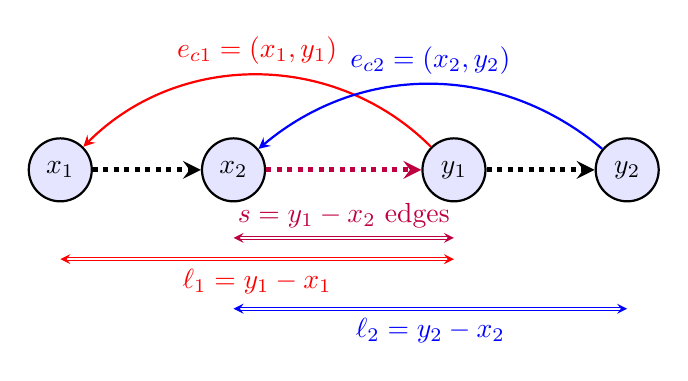
\begin{tikzpicture}[scale=0.9, >=stealth, main/.style={circle, draw=black, fill=blue!10, thick, inner sep=0pt, minimum size=8mm}]
		% Nodes
		\node[main] (x1) {$x_1$};
		\node[main] (x2) [right of=x1, node distance=2.2cm] {$x_2$};
		\node[main] (y1) [right of=x2, node distance=2.8cm] {$y_1$};
		\node[main] (y2) [right of=y1, node distance=2.2cm] {$y_2$};
		
		% Tree Edges
		\draw[dotted,line width=1.8pt, ->] (x1) -- node[above] {} (x2);
		\draw[dotted, line width=1.8pt, purple, ->] (x2) -- node[above, black] {} (y1);
		\draw[dotted,line width=1.8pt, ->] (y1) -- node[above] {} (y2);
		
		% Reverse Cycle Edges
		\draw[thick, red, ->] (y1) to[out=135, in=45] node[above, red] {$e_{c1} = (x_1, y_1)$} (x1);
		\draw[thick, blue, ->] (y2) to[out=140, in=40] node[above, blue] {$e_{c2} = (x_2, y_2)$} (x2);
		
		% Overlap and Length Braces
		\draw[style=double, <->, red] ([yshift=-8mm]x1.south) -- node[below, red] {$\ell_1 = y_1 - x_1$} ([yshift=-8mm]y1.south);
		\draw[style=double, <->, blue] ([yshift=-15mm]x2.south) -- node[below, blue] {$\ell_2 = y_2 - x_2$} ([yshift=-15mm]y2.south);
		\draw[style=double, <->, purple] ([yshift=-5mm]x2.south) -- node[above, purple] {$s = y_1 - x_2$ edges} ([yshift=-5mm]y1.south);
	\end{tikzpicture}
	\caption{Path graph $\mathcal{P}_n$ with two overlapping cycles sharing $s = |\mathcal{E}_{\text{cycle1}} \cap \mathcal{E}_{\text{cycle2}}| > 0$ tree edges.}
	\label{fig:ch_RA_dual_overlapping_cycles}
\end{figure}
\begin{theo}[Non-Overlapping Cycles]\label{nonoverlap}
For two completely non-overlapping cycles ($s = 0$), $D(0) = \frac{\ell_1 + \ell_2 + 2}{(\ell_1+1)(\ell_2+1)} = \frac{1}{\ell_1+1} + \frac{1}{\ell_2+1}$. Under a fixed total cycle edge budget $\ell_1 + \ell_2 = n-1$, $D(0)$ is uniquely minimized when the two non-overlapping cycles are equal in length ($\ell_1 = \ell_2 = \frac{n-1}{2}$ for odd $n$), yielding:
\begin{equation}\label{min_nonoverlap}
	D_{\min} = \begin{cases} \frac{4}{n+1}, & \text{for odd } n \\ \frac{4(n+1)}{n(n+2)}, & \text{for even } n \end{cases}
\end{equation}
\end{theo}

\begin{proof}
Define the continuous function $f(x) \coloneqq \frac{1}{x+1}$ for $x > -1$. Computing derivatives:
\begin{equation}
	f'(x) = -\frac{1}{(x+1)^2}, \quad f''(x) = \frac{2}{(x+1)^3} > 0 \quad \forall x > -1
\end{equation}
Since $f''(x) > 0$, $f(x)$ is strictly convex. By Jensen's Inequality \cite{perlman1974jensen}:
\begin{equation}\label{eq:ch_RA_jensen_proof}
	\frac{f(\ell_1) + f(\ell_2)}{2} \ge f\left( \frac{\ell_1 + \ell_2}{2} \right) \implies \frac{1}{\ell_1+1} + \frac{1}{\ell_2+1} \ge \frac{2}{\frac{\ell_1+\ell_2}{2} + 1} = \frac{4}{\ell_1 + \ell_2 + 2}
\end{equation}
where strict equality holds if and only if $\ell_1 = \ell_2$.

For a path graph on $n$ nodes, non-overlapping cycles span at most $n-1$ total edges ($\ell_1 + \ell_2 \le n-1$). Maximizing total length $\ell_1 + \ell_2 = n-1$ we have:
\begin{enumerate}
	\item \textbf{Odd $n$:} Setting $\ell_1 = \ell_2 = \frac{n-1}{2}$ gives $D_{\min} = \frac{4}{\frac{n-1}{2} + \frac{n-1}{2} + 2} = \frac{4}{n+1}$.
	\item \textbf{Even $n$:} Setting $\ell_1 = \frac{n}{2}$ and $\ell_2 = \frac{n}{2}-1$ gives:
	\begin{equation}
		D_{\min} = \frac{1}{\frac{n}{2}+1} + \frac{1}{\frac{n}{2}} = \frac{2}{n+2} + \frac{2}{n} = \frac{2n + 2(n+2)}{n(n+2)} = \frac{4(n+1)}{n(n+2)}
	\end{equation}
\end{enumerate}
This completes the proof.
\end{proof}
\begin{theo}[$\mathcal{H}_2$ Norm for Two Interacting Cycles]\label{ch_RA_theo2}
Let $\mathcal{P}_n$ be an $n$-node path graph of double integrators containing two interacting cycles of lengths $\ell_1$ and $\ell_2$ sharing $s \ge 0$ edges. The exact $\mathcal{H}_2$ norm of the reduced system $\Sigma$ is:
\begin{align}\label{two_cycle_norm}
	\|\Sigma\|_2^2 = \frac{1}{2\gamma} &\left[ 2\sigma_r^2(n-1) + (\sigma_q^2 + \sigma_r^2)(n - 3 + D) + \sigma_q^2 \frac{(n-1)(n+1)}{6} \right. \nonumber \\
	&\left. + \frac{\sigma_q^2}{d^2} \text{trace}\left( \letree^{-1} (c_1 t_1 t_1^T + c_2 t_1 t_2^T + c_3 t_2 t_1^T + c_4 t_2 t_2^T) \right) \right]
\end{align}
where $T = \begin{bmatrix} t_1 & t_2 \end{bmatrix} \in \mathbb{R}^{(n-1) \times 2}$, and scalar constants $d, D, c_1, c_2, c_3, c_4$ are defined as:
\begin{align}\label{eq:ch_RA_two_cycle_constants}
	d &\coloneqq (\ell_1+1)(\ell_2+1) - s^2, \quad D \coloneqq \frac{\ell_1 + \ell_2 + 2}{d} \nonumber \\
	c_1 &\coloneqq \ell_1(\ell_2+1)^2 - (\ell_2+2)s^2 - 2d(\ell_2+1), \quad c_4 \coloneqq \ell_2(\ell_1+1)^2 - (\ell_1+2)s^2 - 2d(\ell_1+1) \nonumber \\
	c_2 &= c_3 \coloneqq s(s^2 + 2d + 1 - \ell_1 \ell_2)
\end{align}
\end{theo}

\begin{proof}
Consider two cycles represented as, $T = \begin{bmatrix} t_1 & t_2 \end{bmatrix} \in \mathbb{R}^{(n-1) \times 2}$, where $t_1$ and $t_2$ are indicator vectors for Cycle 1 and Cycle 2. The matrix product $T^T T \in \mathbb{R}^{2 \times 2}$ is given by:
\begin{equation}\label{eq:ch_RA_TTT_2cycle}
	T^T T = \begin{bmatrix} t_1^T t_1 & t_1^T t_2 \\ t_2^T t_1 & t_2^T t_2 \end{bmatrix} = \begin{bmatrix} \ell_1 & s \\ s & \ell_2 \end{bmatrix}
\end{equation}

Observe that $I_2 + T^T T = \begin{bmatrix} \ell_1+1 & s \\ s & \ell_2+1 \end{bmatrix}$. Its determinant is $d = \det(I_2 + T^T T) = (\ell_1+1)(\ell_2+1) - s^2$. The inverse is thus given by:
\begin{equation}\label{eq:ch_RA_I_TTT_inv}
	(I_2 + T^T T)^{-1} = \frac{1}{d} \begin{bmatrix} \ell_2+1 & -s \\ -s & \ell_1+1 \end{bmatrix} \eqcolon \begin{bmatrix} a_1 & a_2 \\ a_3 & a_4 \end{bmatrix}
\end{equation}
where $a_1 = \frac{\ell_2+1}{d}$, $a_2 = a_3 = -\frac{s}{d}$, and $a_4 = \frac{\ell_1+1}{d}$.

Applying Woodbury's identity to $(R R^T)^{-1} = (I_{n-1} + T T^T)^{-1} = I_{n-1} - T (I_2 + T^T T)^{-1} T^T$:
\begin{align}\label{eq:ch_RA_RRT_inv_2cycle}
	\text{trace}\left((R R^T)^{-1}\right) &= \text{trace}(I_{n-1}) - \text{trace}\left( T (I_2 + T^T T)^{-1} T^T \right) \nonumber \\
	&= (n-1) - \text{trace}\left( (I_2 + T^T T)^{-1} T^T T \right) \nonumber \\
	&= (n-1) - \text{trace}\left( \frac{1}{d} \begin{bmatrix} \ell_2+1 & -s \\ -s & \ell_1+1 \end{bmatrix} \begin{bmatrix} \ell_1 & s \\ s & \ell_2 \end{bmatrix} \right) \nonumber \\
	&= (n-1) - \frac{(\ell_1(\ell_2+1) - s^2) + (\ell_2(\ell_1+1) - s^2)}{d} \nonumber \\
	&= (n-1) - \frac{2\ell_1 \ell_2 + \ell_1 + \ell_2 - 2s^2}{d} \nonumber \\
	&= n - 3 + \frac{\ell_1 + \ell_2 + 2}{d} = n - 3 + D
\end{align}
where $D = \frac{\ell_1 + \ell_2 + 2}{d}$.

Next, evaluate $(R R^T)^{-2} \letree^{-1} = \left[ I_{n-1} - T (I_2 + T^T T)^{-1} T^T \right]^2 \letree^{-1}$:
\begin{align}\label{eq:ch_RA_RRT_sq_2cycle}
	(R R^T)^{-2} \letree^{-1} &= \letree^{-1} - 2 T (I_2 + T^T T)^{-1} T^T \letree^{-1} + T (I_2 + T^T T)^{-1} T^T T (I_2 + T^T T)^{-1} T^T \letree^{-1} \nonumber \\
	&= \letree^{-1} + T \left[ (I_2 + T^T T)^{-1} T^T T (I_2 + T^T T)^{-1} - 2 (I_2 + T^T T)^{-1} \right] T^T \letree^{-1}
\end{align}

Defining matrix $B_{\text{mid}} \coloneqq (I_2 + T^T T)^{-1} T^T T (I_2 + T^T T)^{-1} = \begin{bmatrix} b_1 & b_2 \\ b_3 & b_4 \end{bmatrix}$ yields:
\begin{align}\label{eq:ch_RA_b_coefficients}
	b_1 &= \frac{\ell_1(\ell_2+1)^2 - (\ell_2+2)s^2}{d^2} \nonumber \\
	b_2 = b_3 &= \frac{s(s^2 + s - \ell_1 \ell_2)}{d^2} \nonumber \\
	b_4 &= \frac{\ell_2(\ell_1+1)^2 - (\ell_1+2)s^2}{d^2}
\end{align}
Defining $c_i \coloneqq d^2 (b_i - 2a_i)$ for $i \in \{1, 2, 3, 4\}$ gives the explicit expressions in \eqref{eq:ch_RA_two_cycle_constants}. Substituting $M_c = \sum_{i,j} c_{i,j} t_i t_j^T$ into the trace equation produces \eqref{two_cycle_norm}, thereby completing the proof.
\end{proof}

When process noise is zero ($\sigma_q = 0$), expression \eqref{two_cycle_norm} simplifies to:
\begin{equation}\label{eq:ch_RA_norm_edge_noise_only}
	\|\Sigma\|_{\sigma_q=0}^2 = \frac{\sigma_r^2}{2\gamma} \left[ 2(n-1) + n - 3 + D \right] = \frac{\sigma_r^2}{2\gamma} \left( 3n - 5 + D \right).
\end{equation}
Under edge noise alone, performance is governed solely by the scalar $D(s, \ell_1, \ell_2) \coloneqq \frac{\ell_1 + \ell_2 + 2}{(\ell_1+1)(\ell_2+1) - s^2}$. Minimizing $\|\Sigma\|_2^2$ is thus equivalent to minimizing $D(s, \ell_1, \ell_2)$.
\begin{comment}
\begin{theo}\label{overlap}
Given an undirected path graph of double integrators on $n$ nodes ($n>4$), suppose two interacting cycles of lengths $\ell_1$ and $\ell_2$ with $s$ shared edges between them results from the addition of two edges. Then, there exist $s>0$ for which the $D \le D_{\min}$, where, $D_{\min}$ is given in \eqref{min_nonoverlap}.
\end{theo}
\end{comment}
Having established that the optimal performance achievable with two non-overlapping cycles occurs when $\ell_1 = \ell_2 = \frac{n-1}{2}$ for odd $n$ (and $\ell_1 = \frac{n}{2}, \ell_2 = \frac{n}{2}-1$ for even $n$), a natural question arises: can introducing spatial overlap between these two cycles enhance $\mathcal{H}_2$ performance even further? The following result addresses this question by establishing exact bounds on the extent of edge overlap that guarantees superior disturbance rejection compared to the optimal non-overlapping baseline established above.
\begin{theo}\label{overlap}
Consider an undirected path graph of double integrators on $n$ nodes ($n > 4$) containing two interacting cycles of lengths $\ell_1$ and $\ell_2$ sharing $s \ge 0$ tree edges resulting from the addition of two cycle-closing edges. Let $D(s)$ denote the performance scalar:
\begin{equation}\label{eq:ch_RA_Ds_def}
	D(s) \coloneqq \frac{\ell_1 + \ell_2 + 2}{(\ell_1+1)(\ell_2+1) - s^2}.
\end{equation}
Furthermore, let the baseline non-overlapping configuration ($s = 0$) span the total edge budget $\ell_1 + \ell_2 = n-1$ such that:
\begin{equation}\label{eq:ch_RA_baseline_lengths}
	(\ell_1, \ell_2) = \begin{cases} \left(\frac{n-1}{2}, \frac{n-1}{2}\right), & \text{for odd } n, \\[6pt] \left(\frac{n}{2}, \frac{n}{2}-1\right), & \text{for even } n, \end{cases}
\end{equation}
which achieves the baseline minimum scalar:
\begin{equation}
	D_{\min} \coloneqq \begin{cases} \frac{4}{n+1}, & \text{for odd } n, \\[6pt] \frac{4(n+1)}{n(n+2)}, & \text{for even } n. \end{cases}
\end{equation}
Then, there exists a non-trivial edge overlap $s > 0$ achieved by expanding the cycle lengths beyond their baseline values \eqref{eq:ch_RA_baseline_lengths} such that $D(s) \le D_{\min}$. Specifically, performance improvement ($D(s) \le D_{\min}$) is guaranteed whenever the spatial overlap increments $k_1$ and $k_2$ (where $s = k_1 + k_2$) satisfy:
\begin{enumerate}
	\item \textbf{For odd $n$:}
	\begin{equation}\label{odd_minD}
		\frac{k_1^2 + k_2^2 + k_1 k_2}{k_1 + k_2} \le \frac{n+1}{4}.
	\end{equation}
	\item \textbf{For even $n$:}
	\begin{equation}\label{even_minD}
		\frac{k_1^2 + k_2^2 + k_1 k_2}{k_1 + k_2} - \frac{k_2}{k_1 + k_2} \le \frac{n^2}{4(n+1)}.
	\end{equation}
\end{enumerate}
\end{theo}
\begin{proof}
Case (1): When $n$ is odd. For non-overlapping case as base case as shown in Figure \ref{fig:ch_RA_base_case_odd_nodes}, we proved in Theorem \ref{nonoverlap} that $D_{\min}=\frac{4}{n+1}$. Now, Let $\ell_1=\frac{n-1}{2}+k_1$ and $\ell_2=\frac{n-1}{2}+k_2$ such that $s=k_1+k_2$ as shown in Figure \ref{fig:ch_RA_overlap_case_odd_nodes}. Thus,
\small
\begin{equation}
	D=\frac{n+1+k_1+k_2}{\frac{(n+1)^2}{4}+(k_1+k_2)\frac{n+1}{2}-k_1^2-k_2^2-k_1k_2}
\end{equation}
\normalsize
\begin{figure}[htbp]
	\centering
	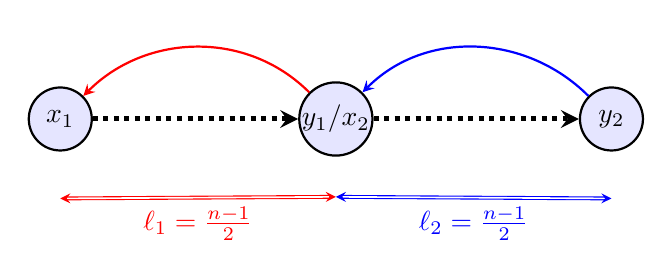
\begin{tikzpicture}[scale=0.85, >=stealth, main/.style={circle, draw=black, fill=blue!10, thick, inner sep=0pt, minimum size=8mm}]
		% Nodes
		\node[main] (x1) {$x_1$};
		\node[main] (y1x2) [right of=x1, node distance=3.5cm] {$y_1$/$x_2$};
		\node[main] (y2) [right of=y1x2, node distance=3.5cm] {$y_2$};
		
		% Spanning Tree Edges
		\draw[dotted,line width=1.8pt, ->] (x1) -- node[above] {} (y1x2);
		\draw[dotted,line width=1.8pt, ->] (y1x2) -- node[above] {} (y2);
		
		% Reverse Cycle Edges
		\draw[thick, red, ->] (y1x2) to[out=135, in=45] node[above, red] {} (x1);
		\draw[thick, blue, ->] (y2) to[out=135, in=45] node[above, blue] {} (y1x2);
		
		% Base Length Braces
		\draw[style=double, <->, red] ([yshift=-7mm]x1.south) -- node[below, red] {$\ell_1 = \frac{n-1}{2}$} ([yshift=-6mm]y1x2.south);
		\draw[style=double, <->, blue] ([yshift=-6mm]y1x2.south) -- node[below, blue] {$\ell_2 = \frac{n-1}{2}$} ([yshift=-7mm]y2.south);
	\end{tikzpicture}
	\caption{Optimal non-overlapping configuration ($s = 0$) for odd $n$, where the cycles meet at node $y_1 = x_2$ without sharing tree edges.}
	\label{fig:ch_RA_base_case_odd_nodes}
\end{figure}
\begin{figure}[htbp]
	\centering
	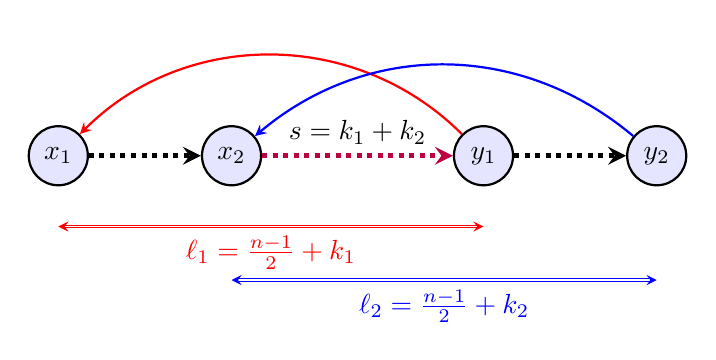
\begin{tikzpicture}[scale=0.85, >=stealth, main/.style={circle, draw=black, fill=blue!10, thick, inner sep=0pt, minimum size=7.5mm}]
		% Nodes
		\node[main] (x1) {$x_1$};
		\node[main] (x2) [right of=x1, node distance=2.2cm] {$x_2$};
		\node[main] (y1) [right of=x2, node distance=3.2cm] {$y_1$};
		\node[main] (y2) [right of=y1, node distance=2.2cm] {$y_2$};
		
		% Spanning Tree Edges
		\draw[dotted,line width=1.8pt, ->] (x1) -- node[above] {} (x2);
		\draw[dotted, line width=1.8pt, purple, ->] (x2) -- node[above, black] {$s = k_1 + k_2$} (y1);
		\draw[dotted,line width=1.8pt, ->] (y1) -- node[above] {} (y2);
		
		% Reverse Cycle Edges
		\draw[thick, red, ->] (y1) to[out=135, in=45] node[above, red] {} (x1);
		\draw[thick, blue, ->] (y2) to[out=140, in=40] node[above, blue] {} (x2);
		
		% Overlap and Expanded Length Braces
		\draw[style=double, <->, red] ([yshift=-6mm]x1.south) -- node[below, red] {$\ell_1 = \frac{n-1}{2} + k_1$} ([yshift=-6mm]y1.south);
		\draw[style=double, <->, blue] ([yshift=-14mm]x2.south) -- node[below, blue] {$\ell_2 = \frac{n-1}{2} + k_2$} ([yshift=-14mm]y2.south);
		%\draw[style=double, <->, purple] ([yshift=-6mm]x2.south) -- node[above, purple] {$s = k_1 + k_2$} ([yshift=-6mm]y1.south);
	\end{tikzpicture}
	\caption{Overlapping configuration showing cycle expansions by $k_1$ and $k_2$ resulting in $s = k_1 + k_2$ shared edges.}
	\label{fig:ch_RA_overlap_case_odd_nodes}
\end{figure}
To minimize it further, $D-D_{\min} \le 0$ needs to be satisfied.
On imposing this requirement, we get 
\begin{equation}
	\frac{k_1^2+k_2^2+k_1k_2}{k_1+k_2} \le \frac{n+1}{4}
\end{equation}
Case 1(a): If $k_1=0$ and $k_2=k$ such that $s=k$, we have
\begin{equation}\label{eq:ch_RA_one_edgeoverlap}
	k \le \frac{n+1}{4}
\end{equation}
Because of symmetry of inequality with respect to $k_1$ and $k_2$, same condition occurs if $k_1=k$ and $k_2=0$.

Case 1(b):If $k_1=k_2=k$ such that $s=2k$, then we have
\begin{equation}\label{eq:ch_RA_equal_edgeoverlap}
	k \le \frac{n+1}{6}
\end{equation}
Case (2): When $n$ is even. Let $\ell_1=\frac{n}{2}+k_1$ and $\ell_2=\frac{n}{2}+k_2-1$, with $s=k_1+k_2$. Thus, we have
\small
\begin{equation*}
	D=\frac{n+1+k_1+k_2}{\frac{n^2}{4}+(k_1+k_2+1)\frac{n}{2}+k_2-k_1^2-k_2^2-k_1k_2}.
\end{equation*}
\normalsize
For base case when $n$ is even, $D_{\min}=\frac{4(n+1)}{n(n+2)}$. To minimize it further, $D-D_{\min} \le 0$ needs to be satisfied.
On imposing this, we get 
\begin{equation}
	\frac{k_1^2+k_2^2+k_1k_2}{k_1+k_2}-\frac{k_2}{k_1+k_2} \le \frac{n^2}{4(n+1)}.
\end{equation}
Case 2(a): If $k_1=0$ and $k_2=k$ such that $s=k$, we have
\begin{equation}
	k \le \frac{n^2}{4(n+1)}+1.
\end{equation}

Case 2(b): If $k_2=0$ and $k_1=k$ such that $s=k$, then it follows that
\begin{equation}
	k \le \frac{n^2}{4(n+1)}.
\end{equation}
Case 2(c): If $k_1=k_2=k$ such that $s=2k$, then we have
\begin{equation}
	k \le \frac{1}{6}\left[n+1+\frac{1}{n+1}\right].
\end{equation}
In all the above cases, the upper bound on $k$ is greater than or equal to 1 for $n>4$, this completes the proof.    
\end{proof}
\begin{remark}
Theorem \ref{overlap} indicates that some amount of overlap is always desirable for an improved performance with respect to $\mathcal{H}_2$ metric in presence of two cycles in a graph.
\end{remark}
\begin{remark}
Though the present analysis was done for a network of double integrators, the same analysis is valid for the case of single integrators, under assumption that $\sigma_q=\sigma_r=1$. However, note that the analysis for double integrator is done under zero node noise, whereas it is equivalent to the single integrator case under influence of both kinds of noises, as in \cite{zelazo2013performance}.
\end{remark}

\section{Numerical Validation and Discussions}\label{sec:ch_RA_simulations}

To validate the theoretical bounds derived in Section \ref{sec:ch_RA_CycleAnalysis},extensive numerical simulations were conducted on a 23-node path graph ($\mathcal{P}_{23}$, $n = 23$) consisting of consensus-seeking double-integrator agents under velocity coupling gain $\gamma = 1$. The baseline non-overlapping configuration is established at the theoretical optimum given by Theorem \ref{nonoverlap} for odd $n$: Cycle~1 and Cycle~2 are assigned identical base length $\ell_1=\ell_2=11$, meeting at the central node $y_1 = x_2 = 12$ with zero edge overlap ($s=0$) and subject to process and measurement noise.

\begin{figure}[ht!]
	\centering
	\begin{subfigure}[b]{0.8\textwidth}
		\centering
		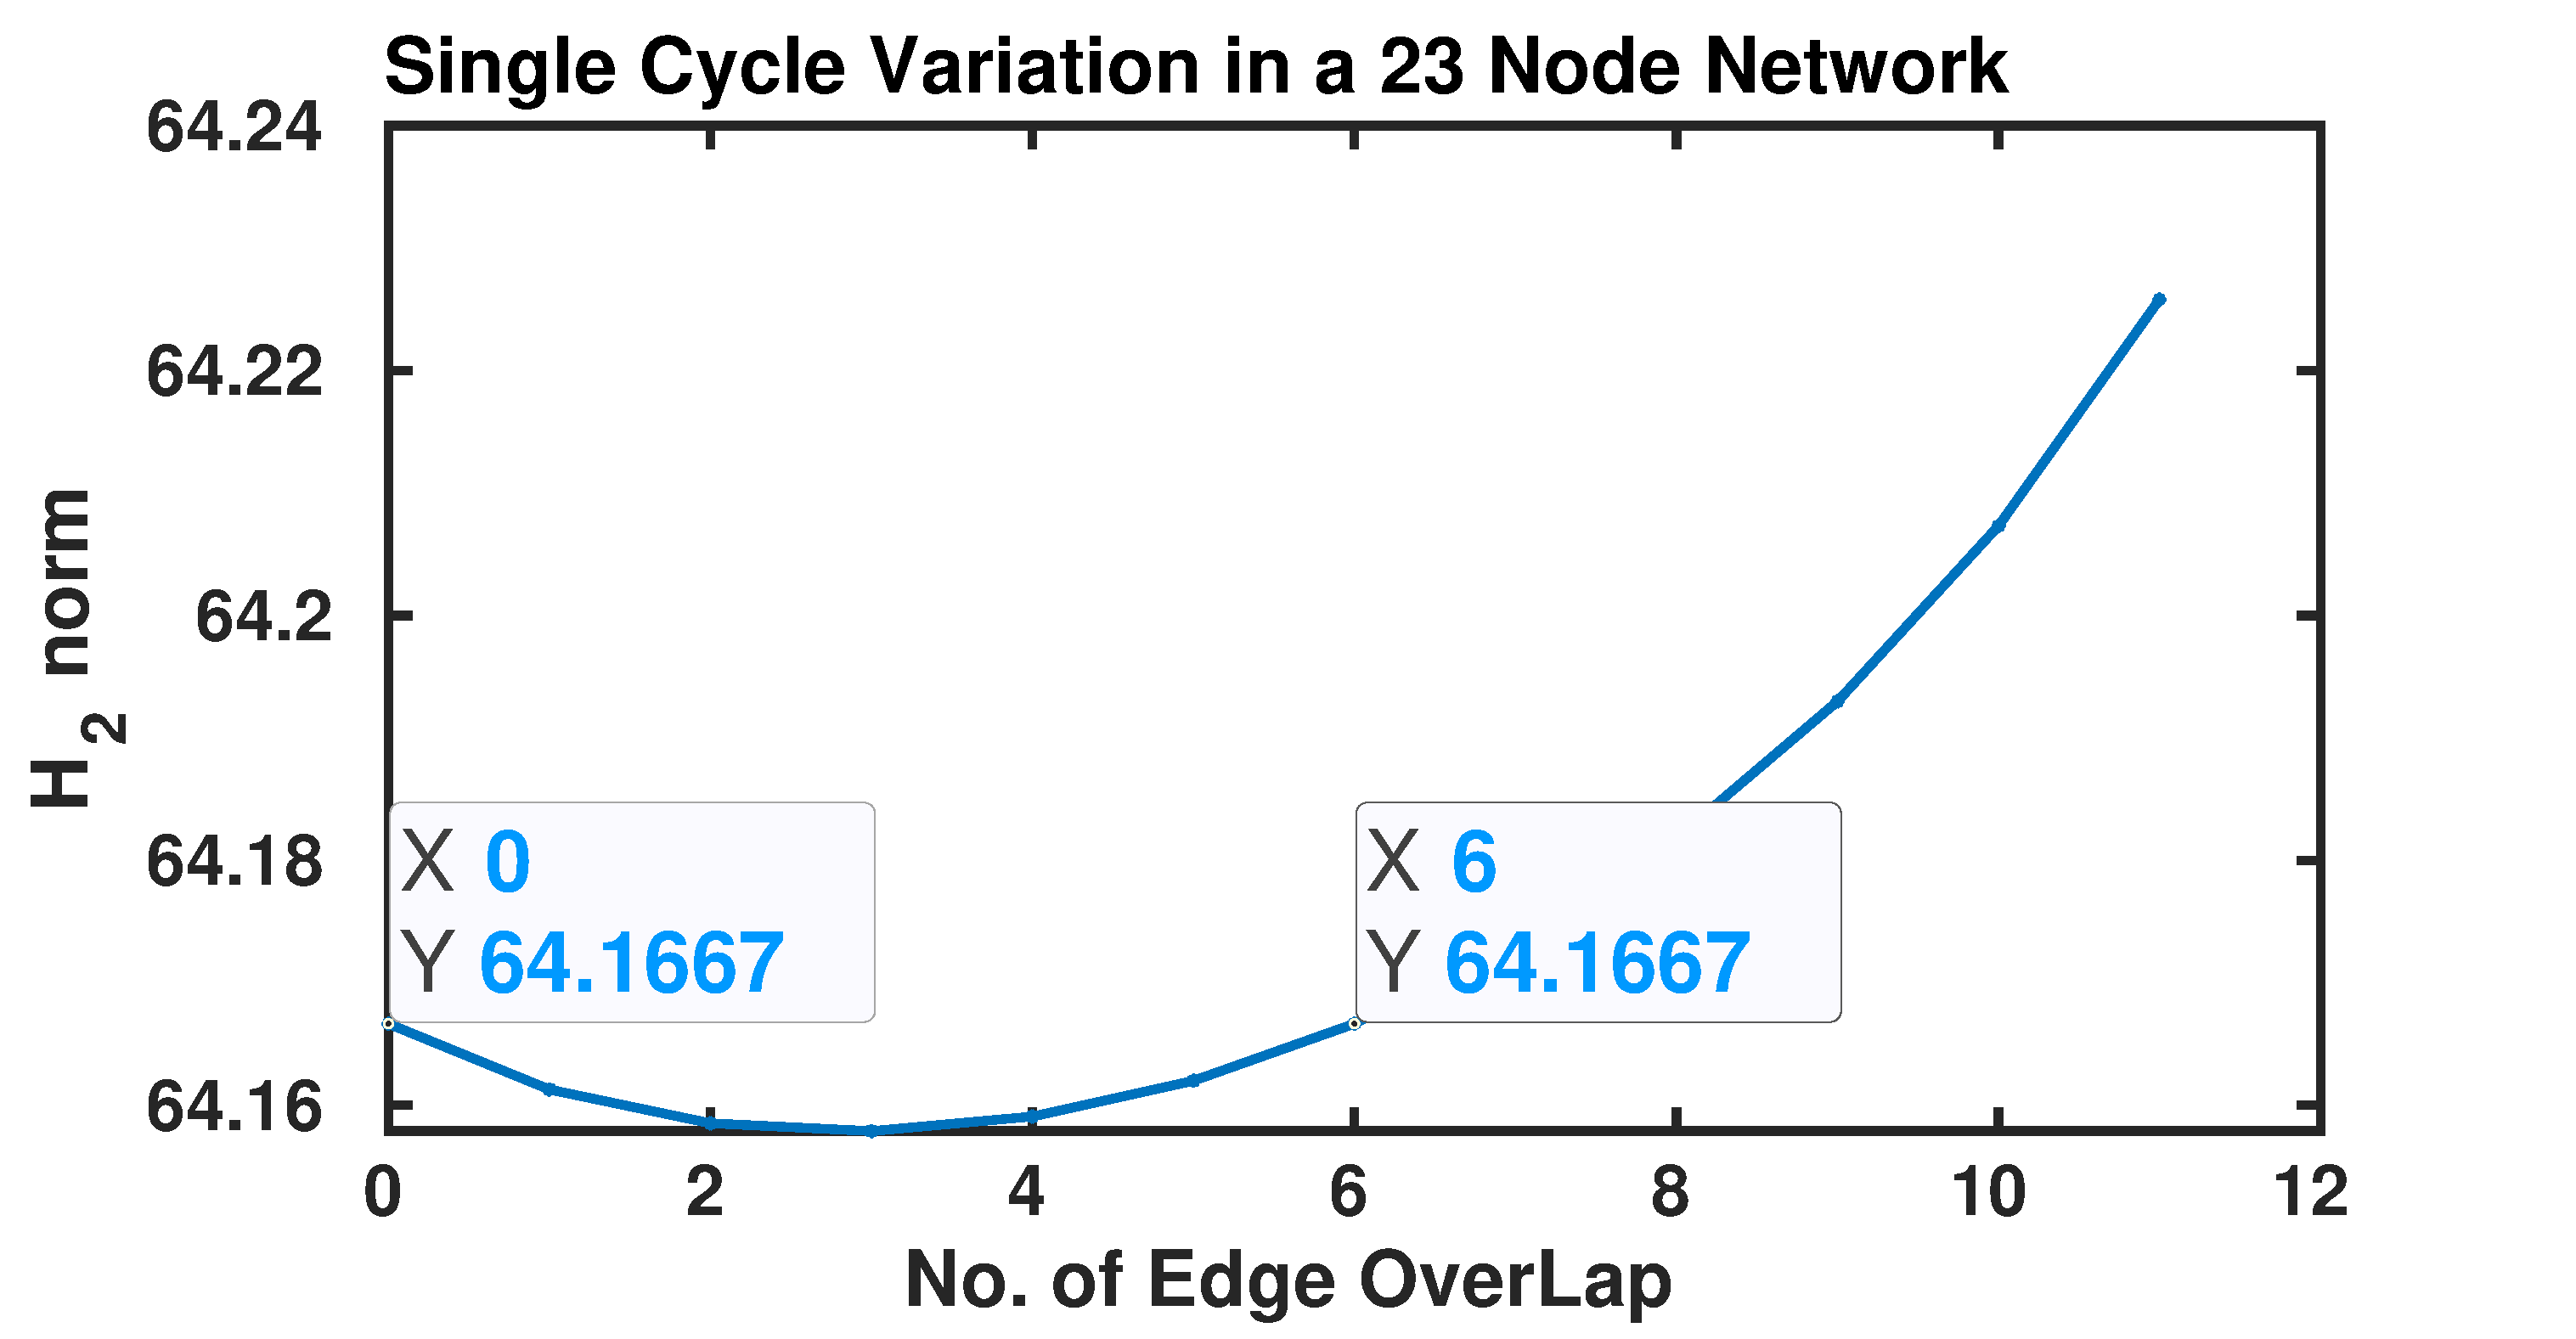
\includegraphics[width=\textwidth, keepaspectratio]{4_Images/Single_Cycle_Variation_23Nodes.eps}
		\caption{Single-cycle length increases by $k$ ($s = k$). Performance improves for $k \le \frac{23+1}{4} = 6$.}
		\label{fig:Single_Cycle_Variation_23Nodes}
	\end{subfigure}
	
	\vspace{1em}
	
	\begin{subfigure}[b]{0.8\textwidth}
		\centering
		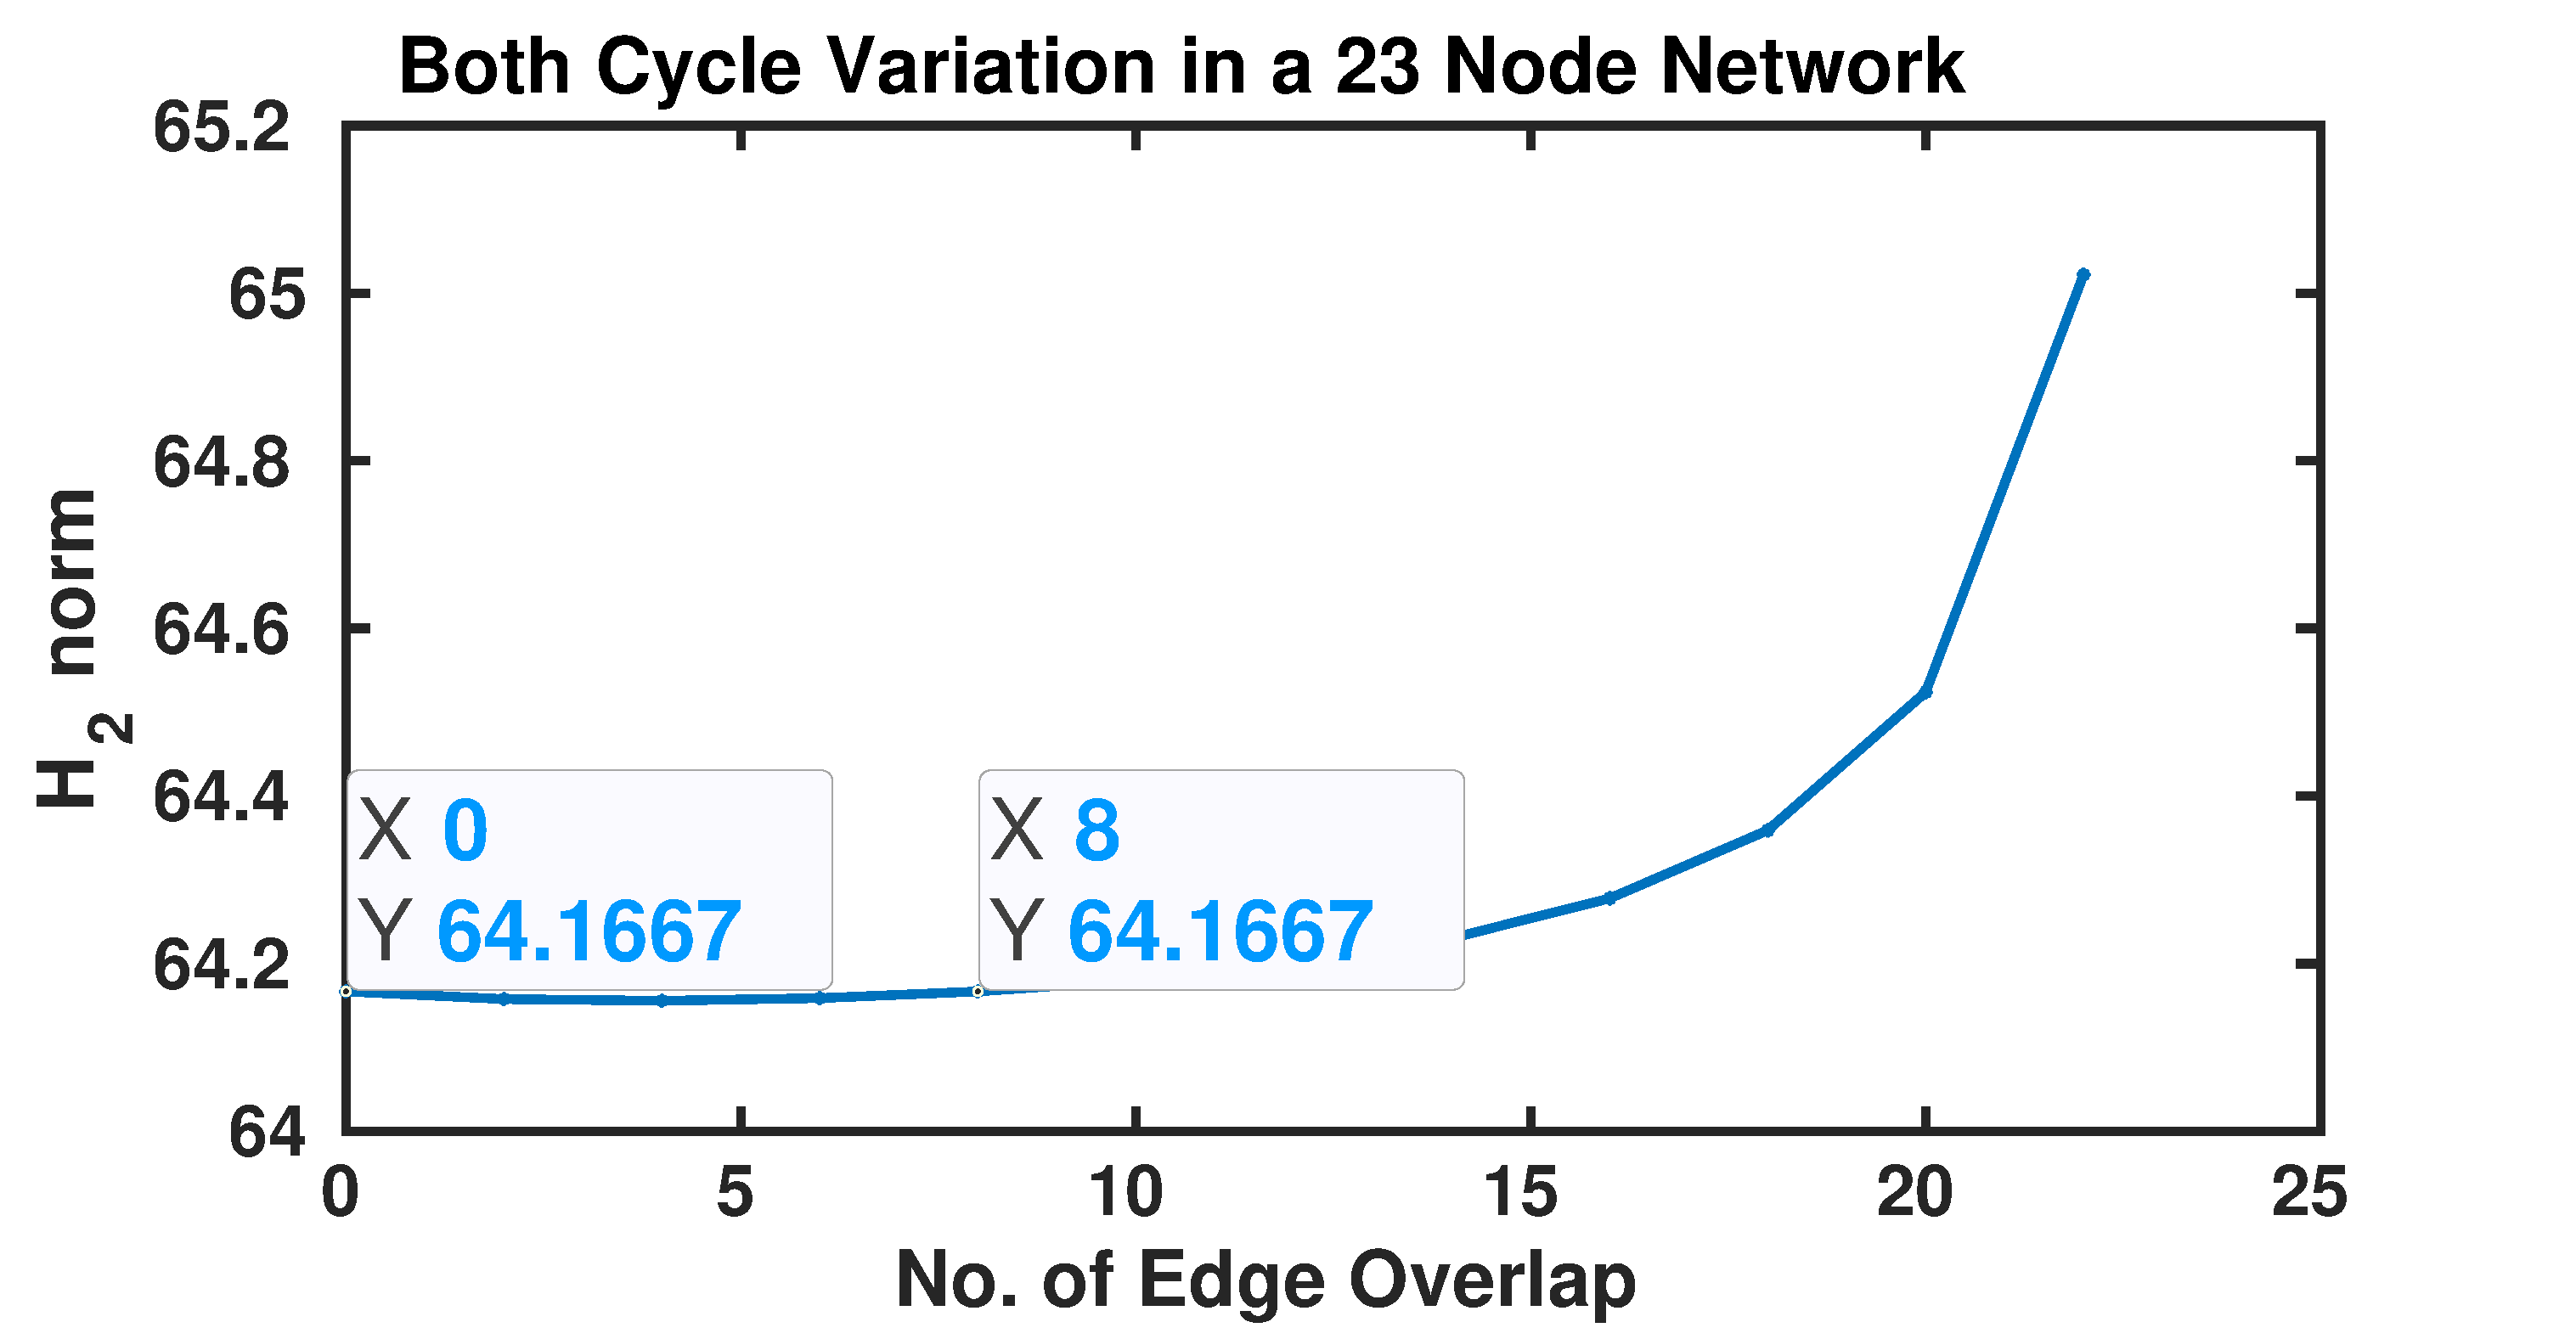
\includegraphics[width=\textwidth, keepaspectratio]{4_Images/Both_Cycle_Variation_23Nodes.eps}
		\caption{Both cycles' length increase by $k$ ($s = 2k$). Performance improves for $k \le \frac{23+1}{6} = 4$.}
		\label{fig:Both_Cycle_Variation_23Nodes}
	\end{subfigure}
	\caption{$\mathcal{H}_2$ norm variation as a function of edge overlap, $s$, between two cycles under measurement noise}
	\label{fig:withedgenoise}
\end{figure}

Figures \ref{fig:Single_Cycle_Variation_23Nodes} and \ref{fig:Both_Cycle_Variation_23Nodes} depict the variation of the system $\mathcal{H}_2$ norm $\|\Sigma\|_2^2$ under pure edge measurement noise ($\sigma_r^2 = 1, \sigma_q^2 = 0$) as a function of the spatial overlap increment $k$. 

In Figure~\ref{fig:Single_Cycle_Variation_23Nodes}, Cycle~1 is expanded by $k$ edges while keeping Cycle~2 fixed at its base length $\ell_2 = 11$, resulting in a direct spatial overlap $s = k$. As predicted by Case~1 of Theorem~\ref{overlap}, introducing edge overlap initially causes the system norm $\|\Sigma\|_2^2$ to decrease monotonically below the non-overlapping baseline $D_{\min}$. The performance metric achieves its global minimum at $k = 6$ ($s = 6$ shared edges), beyond which additional expansion causes $\|\Sigma\|_2^2$ to increase. This matches the analytical upper bound $k_{\max} = \frac{n+1}{4} = \frac{24}{4} = 6$ derived in \eqref{eq:ch_RA_one_edgeoverlap}.


Figure~\ref{fig:Both_Cycle_Variation_23Nodes} illustrates the symmetric dual-cycle expansion scenario, where both cycles are simultaneously expanded by $k$ edges ($\ell_1' = \ell_2' = 11 + k$), generating a mutual overlap $s = 2k$. In strict agreement with Case~2 of Theorem~\ref{overlap}, the $\mathcal{H}_2$ norm improves continuously until $k$ reaches $k_{\max} = \frac{n+1}{6} = \frac{24}{6} = 4$, which corresponds to an optimal shared region of $s = 2(4) = 8$ edges as derived in \eqref{eq:ch_RA_equal_edgeoverlap}. Beyond $k > 4$, excessive structural overlap creates redundant feedback channels that amplify measurement noise propagation, deteriorating overall network performance.

These results validate a fundamental design insight: \textbf{completely non-overlapping loops ($s = 0$) are suboptimal}. A certain degree of structural overlap acts as an algebraic dampener, creating parallel relative-state feedback channels that suppress transient noise energy without overloading the network.

\begin{figure}[ht!]
	\centering
	\begin{subfigure}[b]{0.8\textwidth}
		\centering
		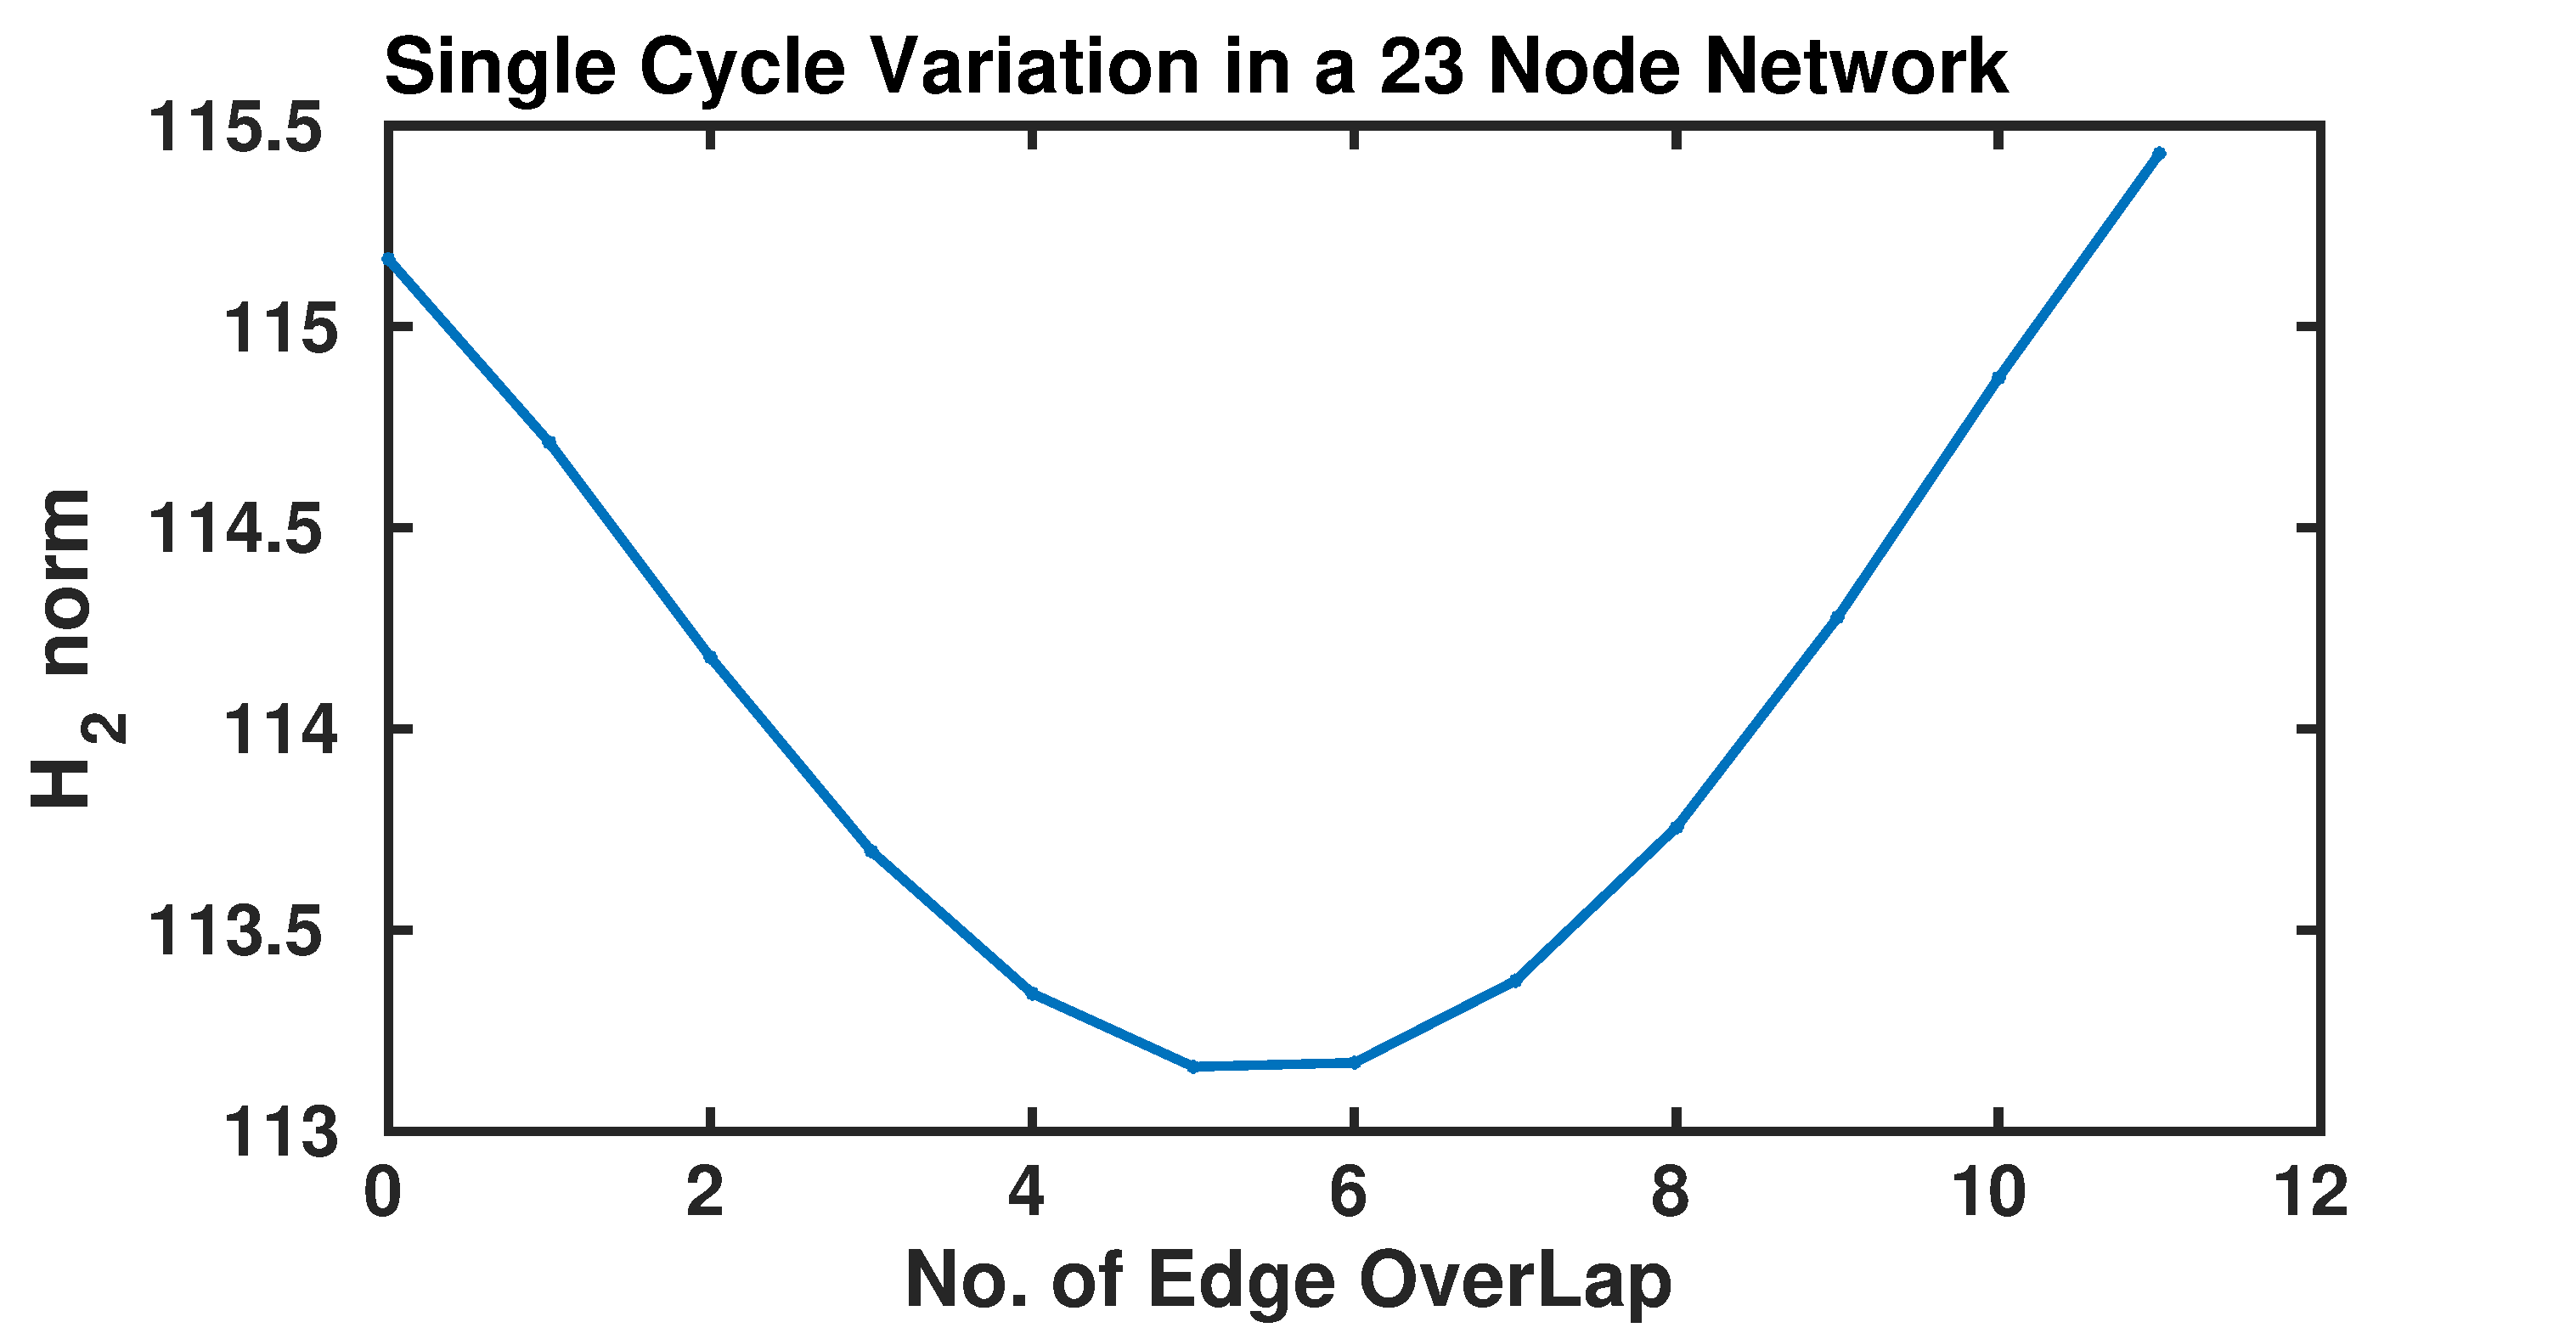
\includegraphics[width=\textwidth, keepaspectratio]{4_Images/Single_Cycle_Variation_23Nodes_BothNoise.eps}
		\caption{Single-cycle length increases under combined noise ($\sigma_q^2 = 1, \sigma_r^2 = 1$).}
		\label{fig:Single_BothNoise}
	\end{subfigure}
	
	\vspace{1em}
	
	\begin{subfigure}[b]{0.8\textwidth}
		\centering
		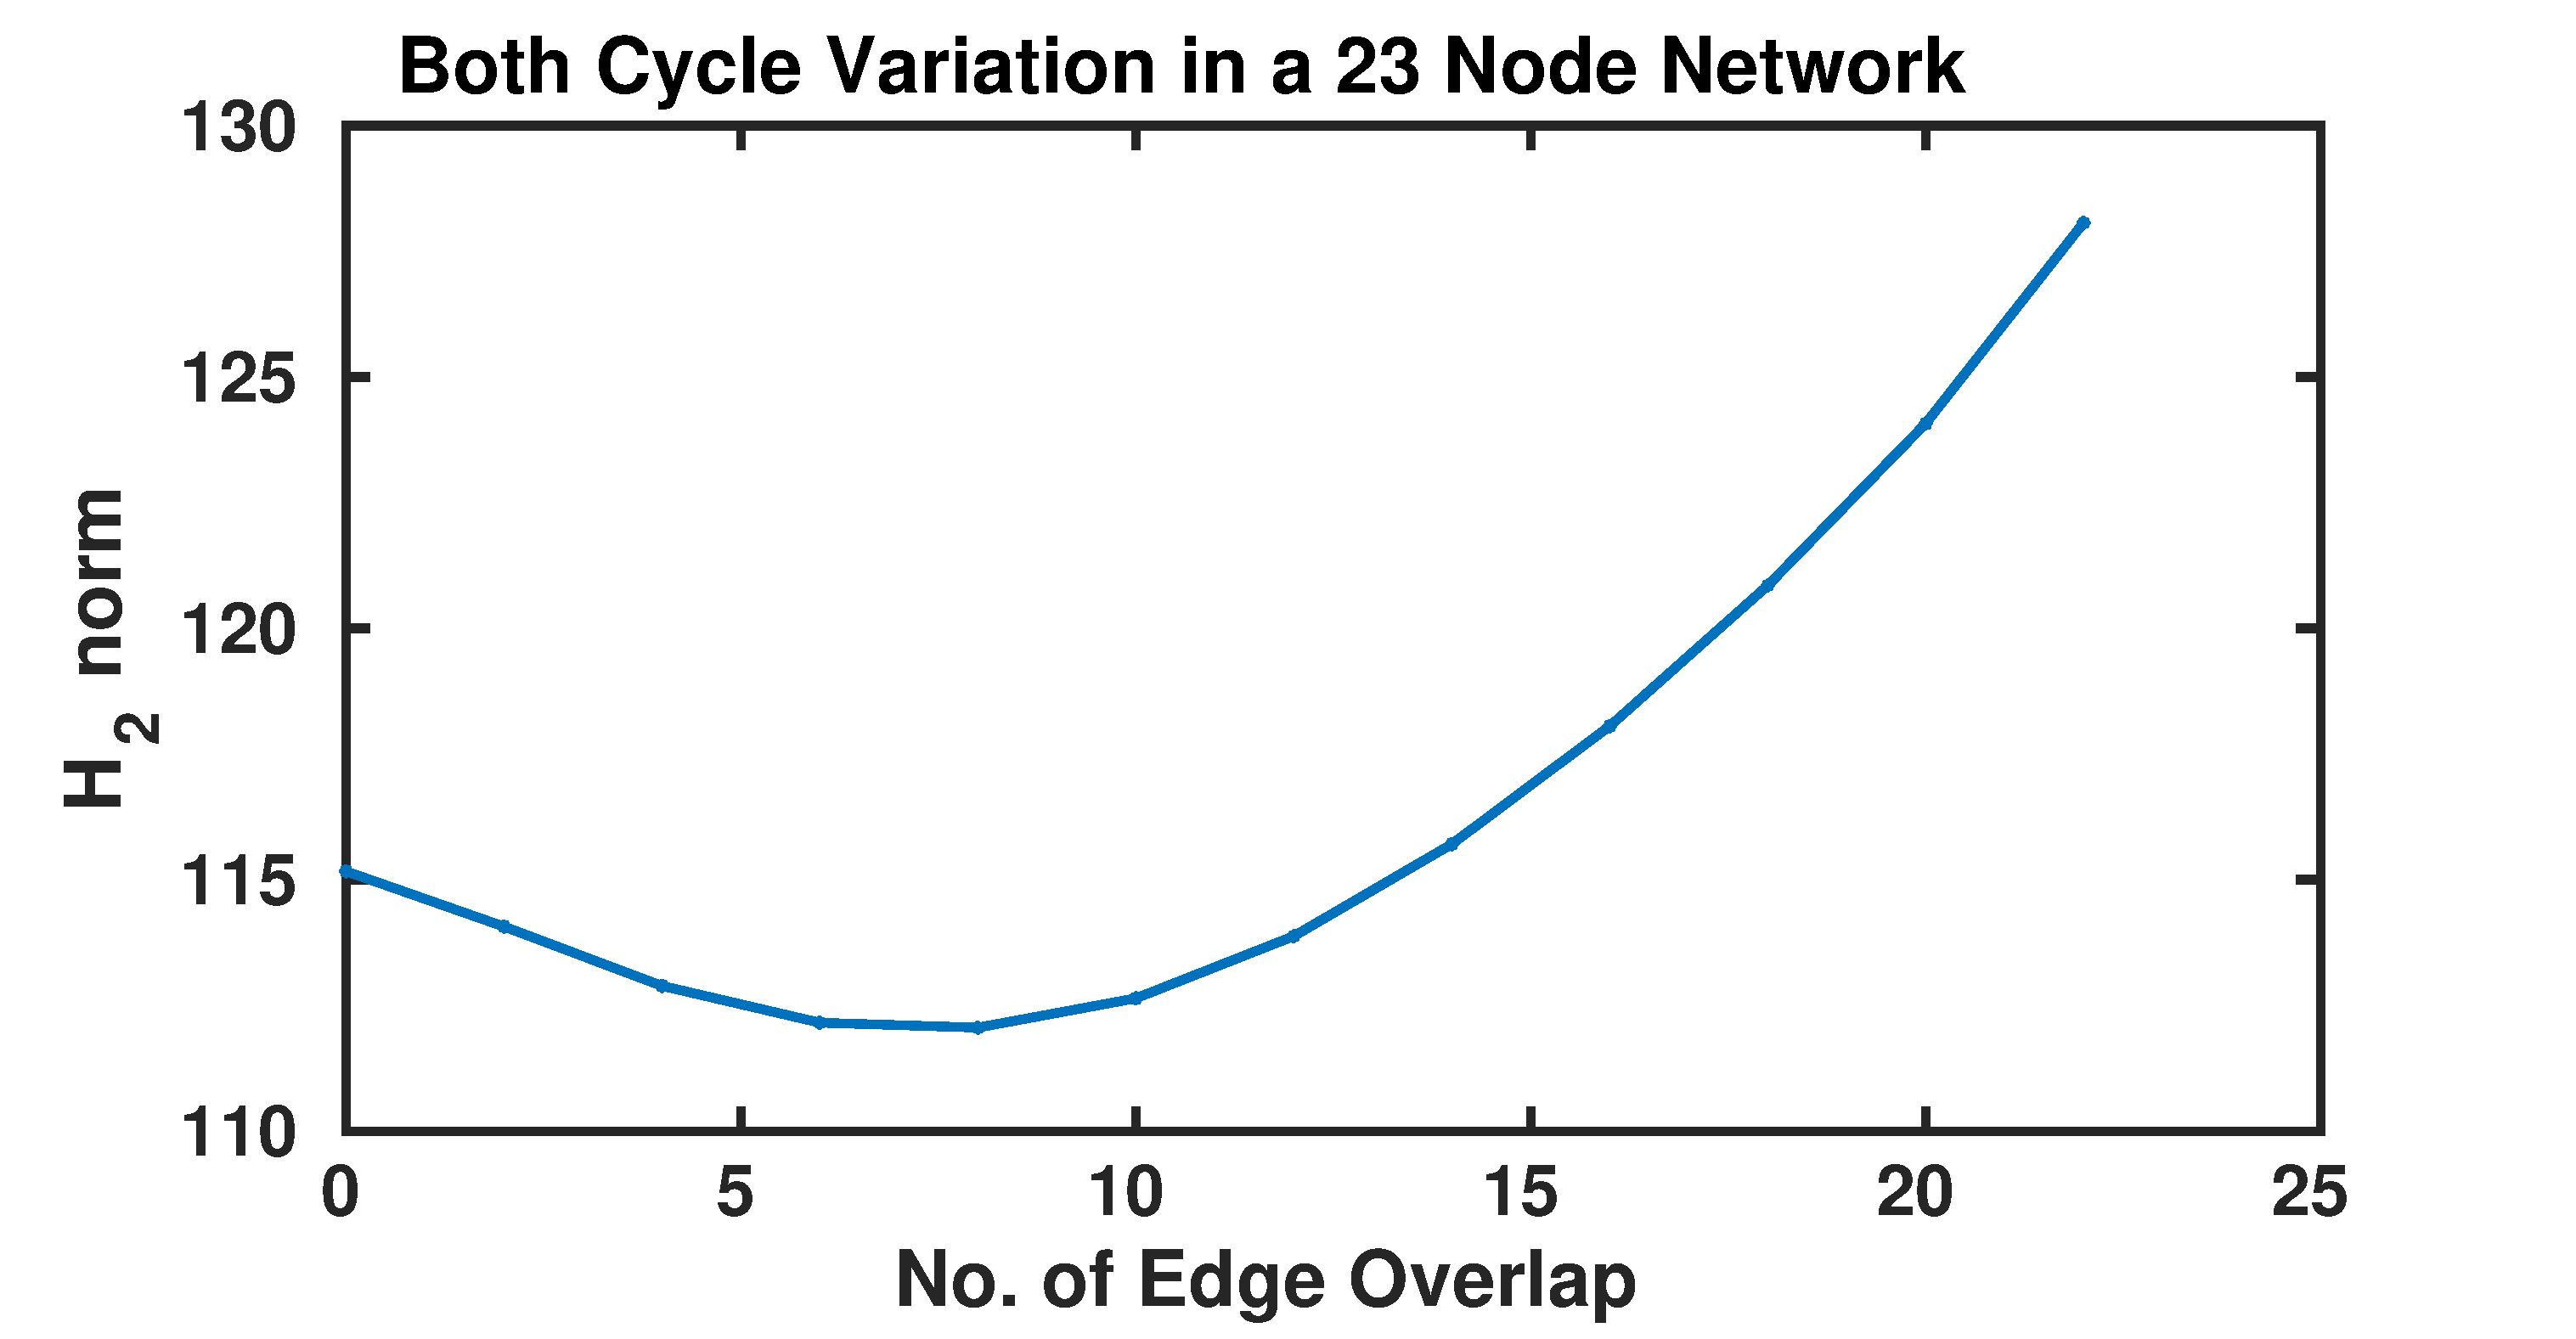
\includegraphics[width=\textwidth, keepaspectratio]{4_Images/Both_Cycle_Variation_23Nodes_BothNoise.eps}
		\caption{Both cycles' lengths increase under combined noise ($\sigma_q^2 = 1, \sigma_r^2 = 1$).}
		\label{fig:Both_BothNoise}
	\end{subfigure}
	\caption{$\mathcal{H}_2$ norm variation with two cycles under combined process and measurement noise.}
	\label{fig:withbothnoise}
\end{figure}

In practical deployments, multi-agent networks operate under simultaneous external process disturbances acting on agent acceleration dynamics ($\sigma_q^2 > 0$) and sensor measurement noise along communication links ($\sigma_r^2 > 0$). Figures~\ref{fig:Single_BothNoise} and \ref{fig:Both_BothNoise} evaluate the $\mathcal{H}_2$ norm under equal process and measurement noise power ($\sigma_q^2 = 1, \sigma_r^2 = 1$).

As observed in Figures~\ref{fig:Single_BothNoise} and \ref{fig:Both_BothNoise}, the addition of process noise scales the overall energy baseline of $\|\Sigma\|_2^2$ due to the persistent excitation of physical velocity states.

Specifically, moderate spatial overlap continues to yield superior disturbance rejection compared to the non-overlapping baseline $s = 0$. The minimum norm regions align closely with the analytical bounds established under pure edge noise, confirming that the optimal overlap bounds derived in Theorem~\ref{overlap} remain robust against process noises.

To validate Theorem~\ref{thm:ch_RA_single_cycle_location}, we analyze the sensitivity of $\|\Sigma\|_2^2$ to the spatial placement of cycle centers across the physical path graph. Figure~\ref{fig:Position_dependence} tracks the $\mathcal{H}_2$ norm across four distinct topological loop-triplet configurations ($\{\ell_1, \ell_2, s\}$) as their spatial anchoring indices are systematically shifted from the boundary nodes toward the graph interior.

The numerical results in Figure~\ref{fig:Position_dependence} demonstrate two critical phenomena:
\begin{enumerate}
	\item \textbf{Monotonic Centering Minimization:} For every tested loop geometry, shifting the cycle anchors closer to the network spatial center $n_c^* = \frac{23+1}{2} = 12$ produces a smooth, monotonic reduction in $\|\Sigma\|_2^2$. Trajectories positioned at the geographic boundaries (near node $1$ or node $23$) exhibit significantly higher noise amplification.
	\item \textbf{Hierarchy of Topological Configurations:} Across all spatial locations, configurations with non-zero edge overlap ($s > 0$) consistently achieve lower $\mathcal{H}_2$ norms than non-overlapping structures ($s = 0$). Specifically, the overlapping configurations $\{\ell_1=3, \ell_2=1, s=1\}$ and $\{\ell_1=4, \ell_2=1, s=1\}$ outperform the non-overlapping baseline $\{\ell_1=1, \ell_2=1, s=0\}$ across every spatial index.
\end{enumerate}

These findings confirm Theorem~\ref{thm:ch_RA_single_cycle_location} and provide some guidelines towards network design for achieving second-order consensus: optimal disturbance rejection requires both spatial centering of feedback loops relative to the graph midpoint and partial structural overlap between adjacent cycles.

\begin{figure}[ht!]
	\centering
	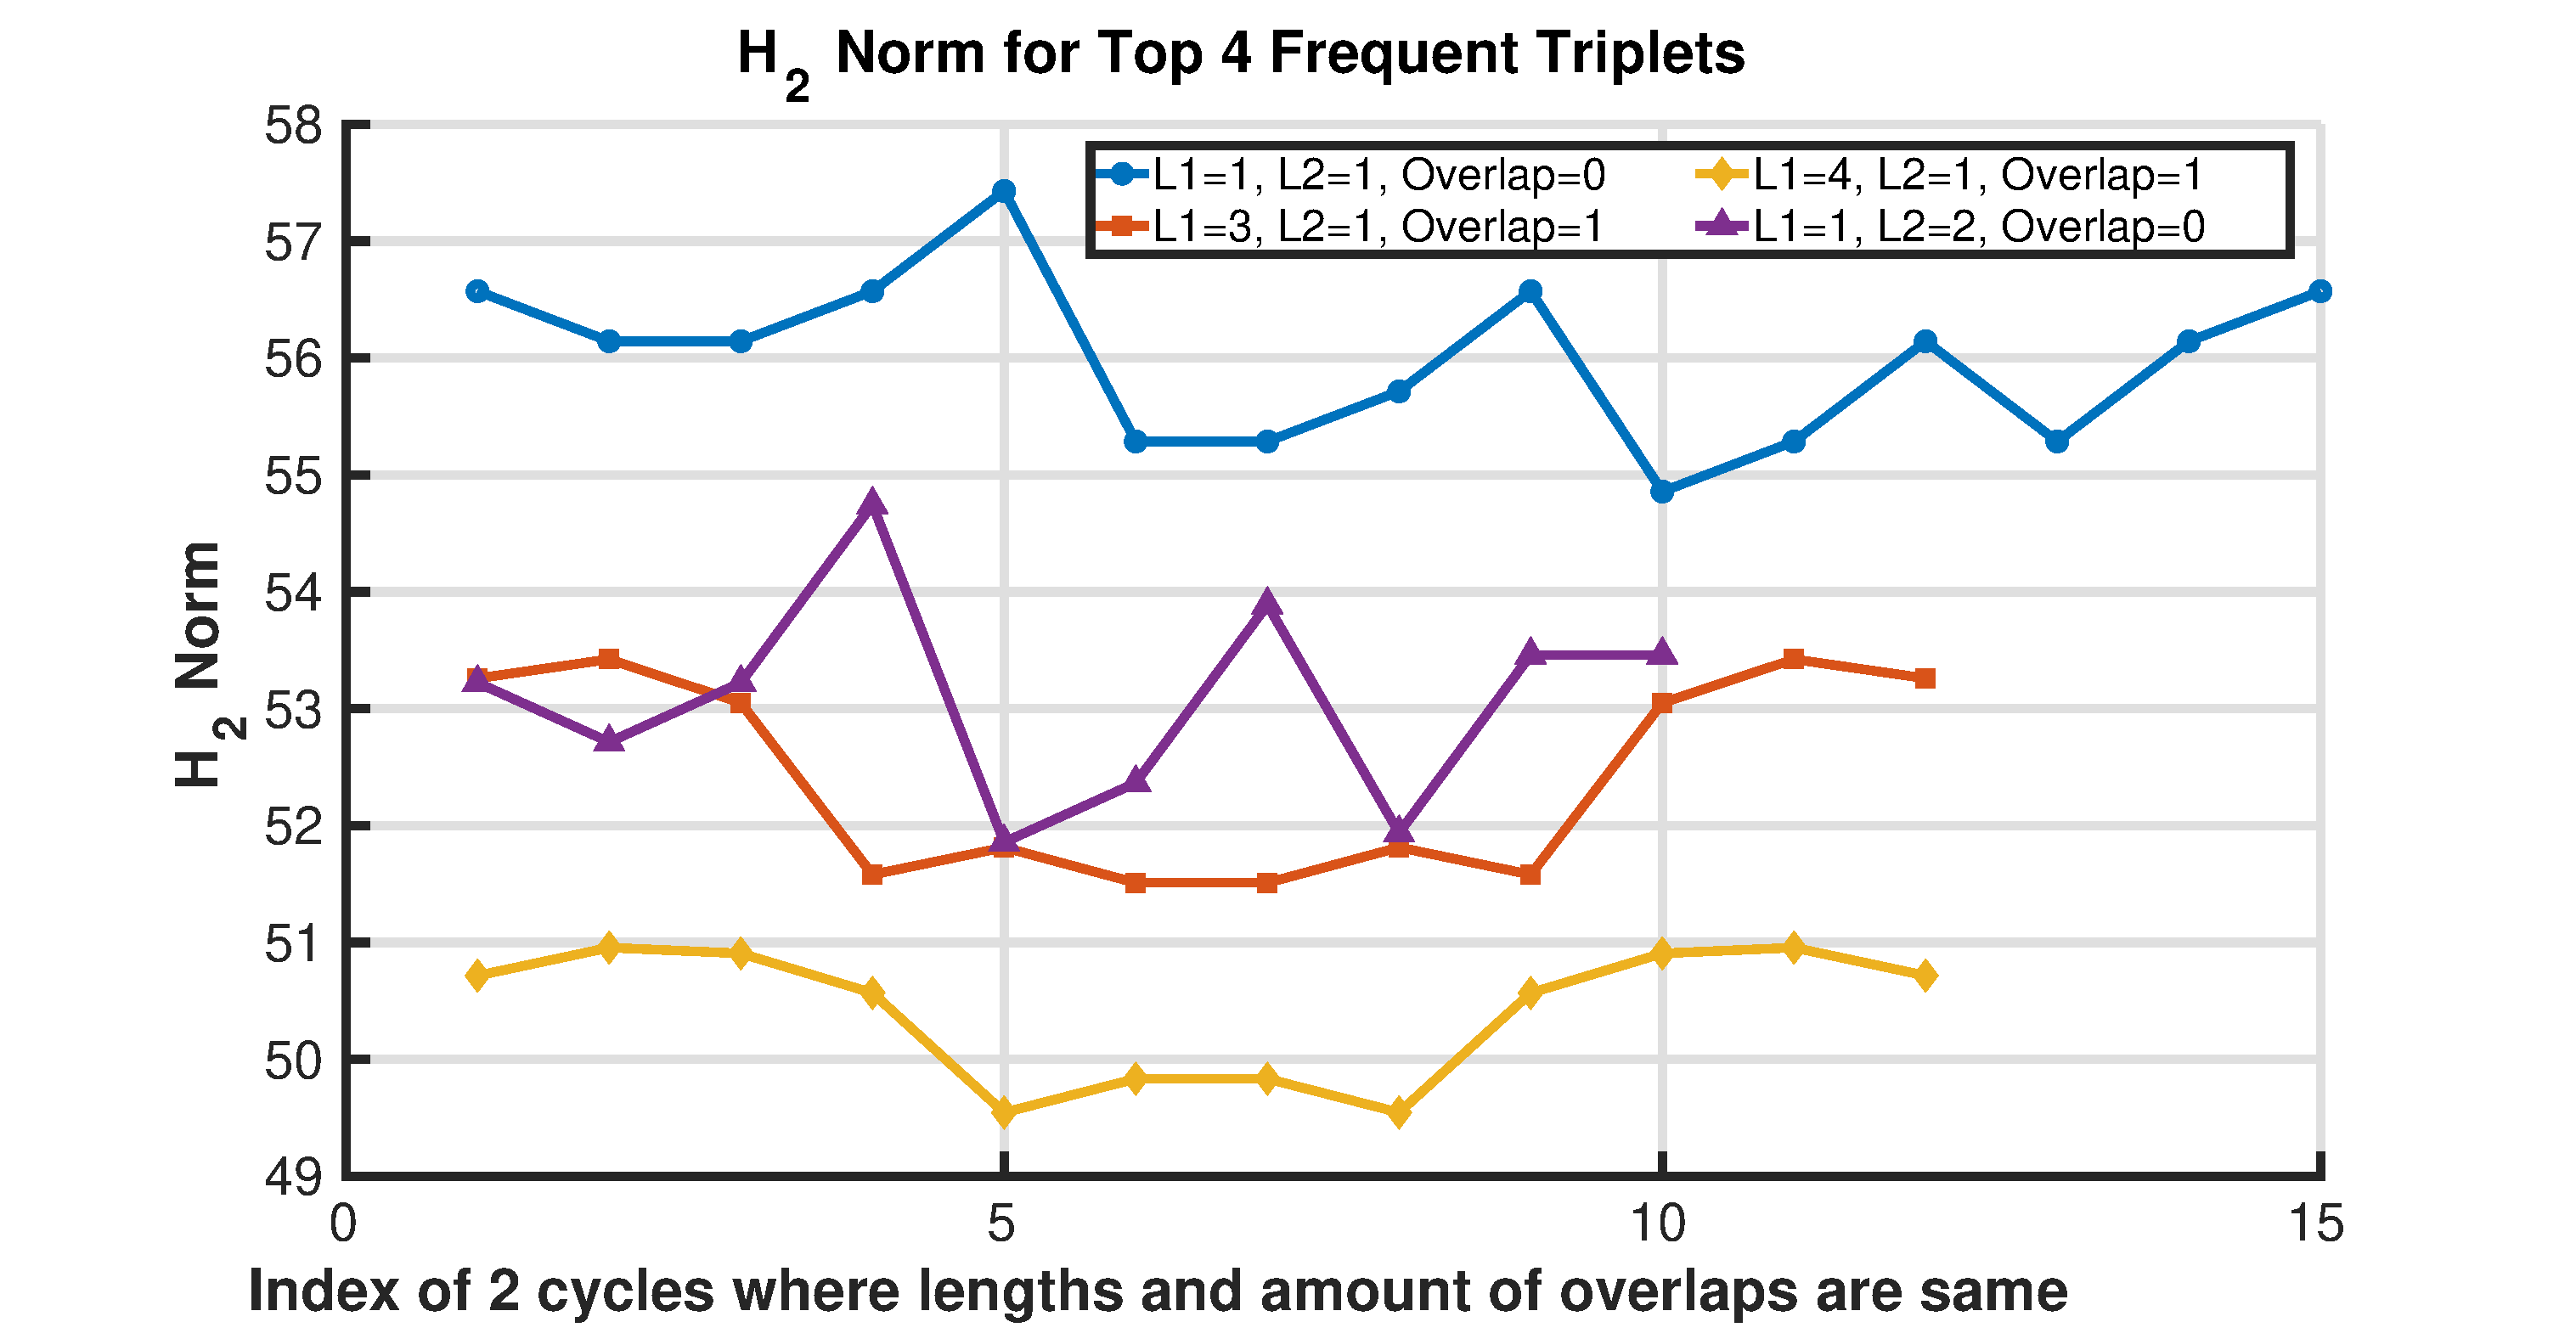
\includegraphics[width=0.8\textwidth, keepaspectratio]{4_Images/PositionalVariation.eps}
	\caption{Spatial position sensitivity: Minimization of $\|\Sigma\|_2^2$ }
	\label{fig:Position_dependence}
\end{figure}


\section{Summary}\label{sec:ch_RA_conclusion}
In this chapter, an analytical $\mathcal{H}_2$ performance framework was formulated for double-integrator multi-agent networks operating over cyclic graphs. The primary analytical conclusions are summarized as follows:

\begin{itemize}
    \item \textbf{Double-Integrator Energy Overhead:} Double-integrator networks inherently store disturbance energy within their physical velocity states ($\text{trace}(X_3) > 0$), resulting in a strictly larger $\mathcal{H}_2$ norm than single-integrator networks operating over identical topologies.
    \item \textbf{Spatial Locality Dependency:} Unlike first-order networks (where all spanning trees and cycle locations yield identical $\mathcal{H}_2$ norms), double-integrator performance depends strictly on the choice of spanning tree and the spatial placement of cycles. Specifically, placing a cycle near the spatial center of a path graph ($n_c = \frac{n+1}{2}$) maximizes systemic noise attenuation.
    \item \textbf{Optimal Cycle Overlap Bounds:} For dual-cycle topologies, moderate edge overlap ($s \le \frac{n+1}{6}$) strictly outperforms completely disjoint cycles, providing optimal noise suppression under environmental process and measurement disturbances.
\end{itemize}
\vspace{0.5em}
\noindent %\textbf{Transition to Chapter 5:}\\
While Chapters \ref{ch:TwoReverseEdges}, \ref{ch:Guaranteed_Consensus}, and \ref{ch:Robustness_Analysis} established exact dynamic consensus boundaries, localized gain tuning remedies, and $\mathcal{H}_2$ noise attenuation metrics across multi-agent communication graphs, real-world autonomous agents (such as mobile robots and unmanned aerial vehicles) must also navigate physical spatial environments under nonholonomic kinematic constraints.

To bridge graph-theoretic cooperative control with real-time physical motion execution, Chapter \ref{ch:Dubins_Path} and \ref{ch:Spiral_Path} shift their focus to local trajectory generation. Specifically, Chapter \ref{ch:Dubins_Path} formulates constrained path planning frameworks utilizing Dubins-like trajectories subject to terminal approach angle and impact time constraints.
